% !TeX program = xelatex
% !TeX encoding = UTF-8
\documentclass[final,5p,times,twocolumn]{elsarticle}

\usepackage{iftex}
\ifXeTeX\else
  \PackageError{JMS_Review_CN}{This manuscript requires XeLaTeX}
    {Select XeLaTeX as the compiler and compile again.}
\fi
\IfFileExists{ctex-fontset-fandol.def}
  {\usepackage[UTF8,scheme=plain,fontset=fandol]{ctex}}
  {\usepackage[UTF8,scheme=plain,fontset=windows]{ctex}}
\usepackage{amsmath,amssymb,mathtools}
\usepackage{booktabs,array}
\usepackage{graphicx}
\usepackage{enumitem}
\usepackage{placeins}
\usepackage{dblfloatfix}
\usepackage{flafter}
\usepackage{microtype}
\usepackage{xurl}
\usepackage{xcolor}
\definecolor{JMSCiteBlue}{HTML}{0072B2}
\usepackage[colorlinks=true,citecolor=JMSCiteBlue,linkcolor=JMSCiteBlue,urlcolor=JMSCiteBlue]{hyperref}
\graphicspath{{./}{revised_figures/}{figures/}{JMS/figures/}}
\setlength{\emergencystretch}{3em}
\setcounter{topnumber}{2}
\setcounter{dbltopnumber}{1}
\setcounter{dblbotnumber}{1}
\renewcommand{\topfraction}{0.90}
\renewcommand{\dbltopfraction}{0.72}
\renewcommand{\textfraction}{0.10}
\renewcommand{\floatpagefraction}{0.90}
\renewcommand{\dblfloatpagefraction}{0.95}

\journal{Journal of Manufacturing Systems（中文审阅稿）}
\biboptions{sort&compress}

\newcommand{\method}{RDMCT-HBS}
\newcommand{\cmax}{C_{\max}}
\newcommand{\pdi}{\mathrm{PDI}}
\newcounter{algorithm}
\newcommand{\algorithmtitle}[1]{\refstepcounter{algorithm}\noindent\textbf{算法~\thealgorithm：#1}\par\smallskip}

\begin{document}
\begin{frontmatter}

\title{面向旋转腔半导体组合设备的系统级调度：
可配置源接口两阶段MILP与结构感知精确搜索}

\author[ustb]{邵立珍（Lizhen Shao）\corref{cor1}}
\ead{lshao@ustb.edu.cn}
\author[ustb]{魏林聪（Lincong Wei）}
\author[ustb]{王蔚（Wei Wang）}

\cortext[cor1]{通讯作者。}
\address[ustb]{北京科技大学控制科学与工程系，北京市海淀区学院路30号，
北京100083，中国}

\begin{abstract}
薄膜制造工艺广泛采用组合设备（cluster tool，CT）在受控真空环境下进行
晶圆加工，其中等离子体增强化学气相沉积（Plasma-Enhanced Chemical Vapor 
Deposition，PECVD）由于空间限制以及工艺需求，多采用旋转式多空间
工艺模块结合辅助晶圆进行满片工艺。本文提出可配置源接口两阶段MILP，以同
一模型表达单源加工和双源混流，并覆盖$4\times1$并行与$2\times2$链式工
艺。第一阶段最小化端到端最大完工时间，第二阶段保持离散排程和当前最大完工时
间并改善加工节拍。为提升有限时间精确搜索，进一步提出结构保持二进制骨架
（SPBS）初始解和结构感知层次割选择算法RDMCT-HBS。实验表明，在
配方未限定模式的8、16、17和20片批次中，纯$4\times1$均取得最短最大完工时间和最高等效吞吐率；相同
600~s预算下，两阶段工作流将四项等待与节拍指标降低39.70\%--94.05\%。SPBS
把限时可行解率由51.67\%提高到100\%，平均PDI降低26.19\%；在共同SPBS的标称实验中，纯SCIP与HEM-13D作为基线，RDMCT-HBS的组件消融用于验证各组成部分的作用与必要性，完整RDMCT-HBS取得最低观察平均PDI和求解时间。该框架在保留求解
器可行性验证、上下界和最优性状态的同时，为双源旋转腔设备提供可复现的系统
级调度方法。
\end{abstract}

\begin{keyword}
半导体制造 \sep 组合设备 \sep 调度 \sep 混合整数线性规划 \sep
分支割 \sep 学习增强精确优化
\end{keyword}

\end{frontmatter}
\section{引言}

半导体制造依赖高资本密度、强自动化的工艺装备，设备利用率与生产节拍不仅取决于腔室加工时间，
还取决于晶圆搬运、腔室占用及控制逻辑之间的协同。CT将多个工艺模块、装载锁和机械手集成在同
一受控环境中；驻留时间、腔室清洗和活动时间波动会进一步压缩可行调度空间\citep{pan2018survey}。
因此，CT 调度并非一般并行机排序问题，而是典型的设备级制造系统协同优化问题。

半导体制造过程中，最重要的三个环节是光刻、刻蚀和沉积，在薄膜沉积环节，能够支持先进制程的
PECVD是现在半导体厂商研究的重点。随着吞吐与空间利用率要求提高，传统CT已经无法满足PECVD的
复杂要求，半导体厂商通过在工艺模块内部布置多个加工空间并引入旋转机构，使得腔室内部旋转交换可
访问空间的位置，来实现在机械手对所有工位可操作的前提下进行多晶圆加工\citep{gu2024applied}。

此外，由于含碳的薄膜难以清洁，多空间旋转腔在加工过程中需保证不存在空的工位，实现满片加工。
为了应对这个问题，半导体厂商提出了可复用辅助PW对多空间旋转腔中空余的工位进行保护，产品晶
圆从大气侧进入，可复用辅助晶圆存储模块直接挂载到真空区，从真空存储区进入，两条物流在旋转腔
汇合并竞争机械手资源，完整拓扑如图~\ref{fig:system-zh-new}。辅助晶圆的引入和腔室满片限制
使得加工方式更加多样，最具代表性的两种工艺模式是$4\times1$并行加工和$2\times2$链式加工。
前者是四个工位并行完成一道工序，后者则是两对晶圆依次完成两道链式工序。
在没有工艺要求的前提下，两种工艺模式会产生不同的效果和吞吐量，需要在相同晶圆数与相同时间参
数下比较纯$4\times1$、纯$2\times2$及两者混跑，才能区分模式本身的效率与混流协调代价。

\begin{figure}[t]
\centering
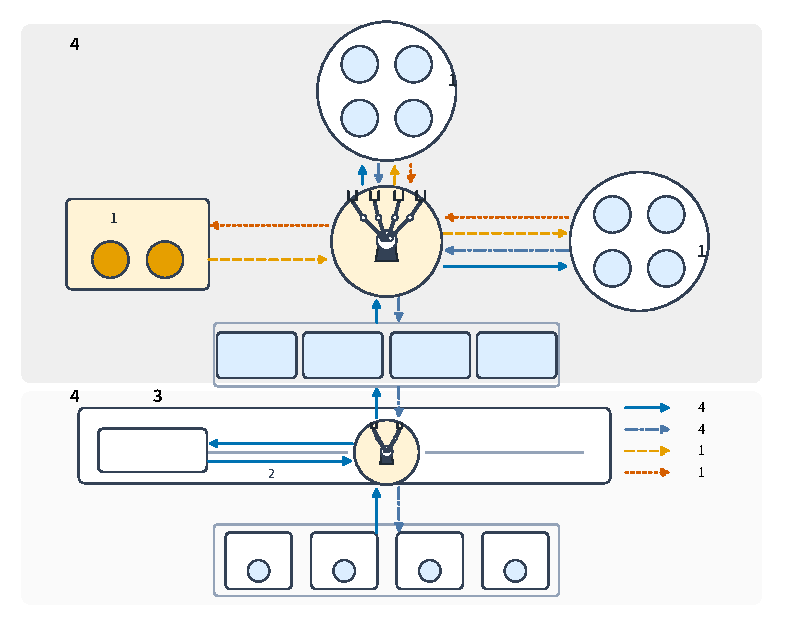
\includegraphics[width=\linewidth]{fig_system_cn}
\caption{双源混流旋转腔组合设备拓扑。产品晶圆由大气侧LP经ATR、AL和LL进入真空域，辅助晶圆由真空存储区经VTR进入旋转腔；实线、点划线、虚线和点线分别表示产品晶圆进片、回片、辅助晶圆进片和回片路径。}
\label{fig:system-zh-new}
\end{figure}

CT调度研究首先围绕吞吐分析和驻留时间可行性展开。\citet{perkinson1994throughput}建立单晶圆CT解析模型，揭示加工时间、搬运时间与最大吞吐率之间的关系。\citet{rostami2002optimal}把工艺模块和搬运模块的驻留约束同时纳入双臂CT调度，并以线性规划结合问题特定启发式求解。\citet{wu2010closedform}基于时间Petri网的稳态排程，推导双臂CT的闭式可调度条件和最优周期排程。\citet{qiao2012sojourn}进一步考虑活动时间有界波动，给出单臂CT晶圆驻留延迟上界及实时控制方法。

随后，研究边界从固定路线扩展到重入工艺与混合生产。\citet{qiao2014revisiting}针对原子层沉积中的重入和驻留约束建立Petri网模型，并得到双臂CT的最优单晶圆循环排程。\citet{wang2020multiple}研究多类晶圆共享双臂CT且同时受驻留时间限制的调度问题。\citet{wang2025virtualcell}提出虚拟单元模型，联合选择启用的工艺模块数量和机械手等待时间，不再预设全部模块必须投入加工。从制造系统层面看，\citet{lee2018waiting}把等待超限与产出率、缓冲容量及上游设备控制联系起来，说明设备级排程在评价系统性能时仍需保留时间窗信息。

随着多品种并行加工、非周期运行和多设备耦合增强，死锁成为CT调度中的关键可行性问题：当晶圆占用工艺模块或缓冲位置并等待机械手，而机械手或相邻资源又被其他晶圆的后续动作占用时，可能形成循环等待，使系统无法继续推进。\citet{zhu2025failuredeadlock}针对带驻留约束的双组合设备故障关机过程，分析相邻机械手在共享缓冲模块处的任务同步关系，并把避免缓冲区死锁的条件嵌入调度模型。\citet{kim2025noncyclicdeadlock}进一步面向多晶圆类型的非周期CT调度，以动态设备状态驱动机械手动作选择，并在决策过程中显式排除会导致死锁的动作。这些近期研究表明，死锁处理正在从依赖固定循环序列，转向对动态状态、共享资源和跨设备同步关系的显式约束。对于本文的双源旋转腔设备，可复用辅助晶圆、四工位满片占用、$4\times1/2\times2$模式切换、清洗任务和共享VTR共同形成跨路线资源耦合，因此需要把死锁避免直接纳入统一的有限批次排程模型。

清洗约束形成了另一条研究主线，因为清洗既占用腔室，又会改变机械手动作序列。\citet{kim2013cleaning}枚举周期清洗下可行的双臂机械手任务序列，并在完全枚举代价过高时采用启发式搜索。\citet{yu2020delay}结合部分装载和机械手任务时刻控制，同时降低带清洗双臂CT的周期时间与晶圆延迟。\citet{qiao2022binary}以虚拟晶圆表示清洗占用，并用二元整数规划优化带驻留约束的双臂CT。\citet{li2022conditioncleaning}把清洗触发与腔室状态关联，推导时间受限单臂CT的可行排程。

近期研究继续向复杂设备结构和混合生产推进。\citet{gu2024multifinger}针对四指机械手和四空间模块，以线性规划求取稳态最小周期。\citet{yang2025miptwowafers}用MIP联合决定两类晶圆投放与机械手动作。这些进展仍未覆盖一个独立的有限批次问题：两个外部源向同一真空域供片，可复用辅助晶圆保证满片加工，且$4\times1$与$2\times2$两种旋转配方并存下的设备调度。

学习型CT控制处于不同的决策层。\citet{kim2025adaptivecluster}用深度强化学习与前瞻搜索选择非周期调度动作。\citet{hong2026ddpgct}在离散事件仿真中用DDPG调节PVD加工时间。与之不同，本文把加工时间视为输入，并要求输出可由MILP验证的完整排程、上下界与最优性状态，因此学习增强精确优化提供了更合适的接口。\citet{tang2020cut}将选割写成强化学习策略。\citet{huang2022cutranking}学习候选割排序。\citet{paulus2022looking}以强前瞻规则生成模仿目标。\citet{wang2023hem}用层次策略联合决定割数量和有序割集。

由此得到两个缺口：设备模型缺少把外部源拓扑、满片模式、辅助晶圆、清洗和共享搬运统一起来的有限时域表达；通用割特征又不能区分离散设备选择、连续事件时刻及其耦合。本文以设备结构贯穿建模、初始解和割选择，贡献为：
\begin{enumerate}[leftmargin=*]
\item 建立可配置源接口两阶段MILP，以同一内部模型表达单源加工和双源混流，并覆盖$4\times1/2\times2$、辅助晶圆、清洗、驻留及共享资源等约束；
\item 提出吞吐优先、运行质量次级的优化机制，在保持离散排程和最大完工时间的条件下减少等待与节拍波动；
\item 提出SPBS初始解与\method{}割选择器；后者在HEM层次数量--序列框架上新增23维角色感知表示、分组门控编码和策略锚定的角色次模补全，并在正式推理中采用束搜索，在不改变MILP可行域和证明逻辑的前提下改善限时原始--对偶搜索。
\end{enumerate}

\section{工业问题建模与两阶段MILP}
\setcounter{equation}{0}

\subsection{针对两种工艺模式需求的PW对建模}

本文建立面向双源混流CT调度问题的有限批次离线排程模型。输入包括产品晶圆数量及工艺模式、设备动作时间、清洗间隔、驻留上限、装载锁容量和辅助晶圆库存；输出包括每片产品晶圆与辅助晶圆的完整路线、每项动作的开始和结束时刻，以及竞争同一物理资源的动作顺序。所有时间参数在一次求解中视为已知，除LP、对准器、装载锁、工艺腔室和辅助晶圆存储区外，不设置额外缓冲区。

PW对（wafer pair）是由两个晶圆组成的物理搬运与腔室占位单元，可由“产品+产品”（产品PW对）、“辅助+辅助”（辅助PW对）或“产品+辅助”（混合PW对）构成。产品晶圆优先按工艺模式和编号两两配成产品PW对；产品数为奇数时，尾片可与一片辅助晶圆形成混合PW对，满片补位与清洗则必须使用辅助PW对。模型中的$\mathcal P^F$和$\mathcal P^L$索引含产品的PW对，包括产品PW对和必要的混合PW对。物理上的单片对准和驻留时间仍逐片建模，对内两片晶圆只在双手ATR、成对搬运选择和相同腔室侧位上共享事件窗口。等价的含产品PW对再按预处理规则固定到规范化候选位置；这只消除编号互换形成的对称解，MILP仍决定有效批次或链位置、辅助晶圆的物理身份、成对搬运选择、共享资源次序和所有事件时刻。清洗位置依据清洗间隔和完整工艺边界预生成，模型再激活相应清洗任务并联合优化其具体时刻。

产品晶圆沿“LP--ATR--AL--ATR--上装载锁--VTR--旋转腔--VTR--下装载锁--ATR--LP”流动，其中ATR先把晶圆放至AL完成校准，再将其取回并送入真空域；辅助晶圆从真空存储区经VTR进入旋转腔，使用结束后经VTR返回原存储区。$4\times1$模式的常规满产品批次由两个产品PW对、即四片产品晶圆组成，四个工位只执行一次同步加工，再按后装先卸顺序取出；末批产品不足时，仅在最后一个有效批次中用辅助PW对或混合PW对补齐四个工位。$2\times2$模式中，每个含产品PW对必须连续出现在相邻两个加工周期中，使其中每片产品晶圆完成两次加工。以三个产品PW对为例，链首先放入辅助PW对D，腔室自转后装入P1并完成“D+P1”腔室加工；随后交替执行腔室加工与“腔室自转+链式滑动”，占位状态依次转为“P1+P2”“P2+P3”和“P3+D”，P1、P2和P3均分别加工两次，最后再取出全部晶圆。图~\ref{fig:chain-zh}和图~\ref{fig:parallel-zh}给出两种模式的事件顺序。

\begin{figure}[t]
\centering
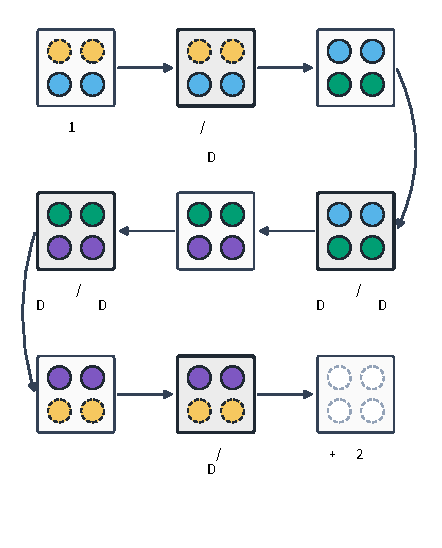
\includegraphics[width=\linewidth]{fig_chain_cn}
\caption{$2\times2$链式加工过程。辅助PW对D在链首与链尾用于保持腔室满片；产品晶圆随腔室旋转和链式滑动依次进入相邻加工周期，每片产品晶圆完成两次加工。}
\label{fig:chain-zh}
\end{figure}

\begin{figure}[t]
\centering
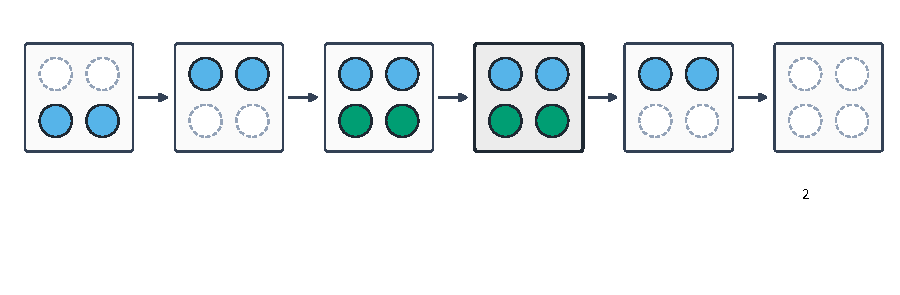
\includegraphics[width=0.94\linewidth]{fig_parallel_cn}
\caption{$4\times1$并行加工过程。两组PW对依次装入旋转腔，四个工位满片后同步加工，并按后装先卸顺序完成卸片；末批不足时由辅助晶圆补齐空余工位。}
\label{fig:parallel-zh}
\end{figure}


\subsection{源接口与基本时间关系}

文中出现的集合与常量如表~\ref{tab:symbol-cn-a}所示，决策变量及辅助变量如表~\ref{tab:symbol-cn-b}所示。

\begin{table*}[t]
\centering
\scriptsize
\setlength{\tabcolsep}{2.5pt}
\caption{集合与参数}
\label{tab:symbol-cn-a}
\begin{tabular}{p{0.20\textwidth}p{0.20\textwidth}p{0.55\textwidth}}
\toprule
符号 & 类型与角色 & 含义 \\
\midrule
$\mathcal S,\mathcal I$ & 集合 & 物料源接口集合与物料单元集合；$i\in\mathcal I$可为产品或辅助晶圆需求。\\
$\mathcal W$ & 集合 & 产品晶圆集合，索引为$w$。\\
$\mathcal P^F,\mathcal P^L$ & 集合 & 分别采用$4\times1$和$2\times2$工艺的含产品PW对集合，索引为$p$。\\
$\mathcal C$ & 集合 & 旋转工艺腔室集合，索引为$c$。\\
$\mathcal B_c,\mathcal K_c$ & 有序集合 & 腔室$c$的$4\times1$候选批次$b$和$2\times2$产品链位置$k$。\\
$\mathcal L=\{1,2\}$ & 集合 & $4\times1$批次的前、后两侧。\\
$\mathcal Q_c,\mathcal E_c$ & 有序集合 & 腔室$c$的$2\times2$加工周期$q$与清洗区段$e$。\\
$\mathcal V_c$ & 集合 & 腔室$c$中所有$4\times1$批次与$2\times2$加工周期的并集。\\
$\mathcal O,\mathcal A$ & 集合 & 候选物理操作集合与必须满足的工艺先后弧集合。\\
$\mathcal R,\Lambda_r$ & 集合 & 共享资源集合及资源$r$的物理槽位集合。\\
$\mathcal J_c^D,\mathcal T_c$ & 集合 & 腔室$c$的辅助晶圆需求集合与可复用物理辅助晶圆集合。\\
$\chi_{is}$ & 0-1常量 & 物料单元$i$是否属于源接口$s$。\\
$\bar x^F_{pcbl},\bar x^L_{pck}$ & 0-1常量 & 对称破除后，PW对与$4\times1$批次侧位或$2\times2$链位置的规范化对应。\\
$q_c^-(k),q_c^+(k)$ & 非负整数常量 & $2\times2$链位置$k$对应的第一次和第二次加工周期，满足$q_c^+(k)=q_c^-(k)+1$。\\
$\bar z_{ce},\bar a^F_{cbe},\bar a^L_{cqe}$ & 0-1常量 & 预生成清洗布局中的有效区段、$4\times1$批次所属区段和$2\times2$周期所属区段。\\
$H,\bar Q_c$ & 非负整数常量 & 相邻清洗间最大有效加工数，以及规范化布局生成的$2\times2$有效周期数。\\
$d_o,\delta_{oo'}$ & 非负连续常量 & 操作$o$的持续时间及先后弧$(o,o')$要求的最小间隔。\\
$d^F_\nu,d^L,r_c$ & 非负连续常量 & $4\times1$阶段$\nu$的时间、$2\times2$加工时间及腔室半周旋转时间。\\
$\rho^r_{oo'}$ & 非负连续常量 & 资源$r$从操作$o$终点空载移动或复位到$o'$起点所需时间。\\
$M,\overline R_{wr}$ & 正连续常量 & 有效大常数上界，以及晶圆$w$在受限区段$r$中的最大驻留时间。\\
$\kappa_o,\Gamma_o$ & 整数常量/集合 & 操作$o$需要的资源占用单元数及允许使用的占用单元集合；对ATR、VTR和腔室表示执行机构互斥单元，对装载锁和辅助晶圆库存表示物理槽位或物理身份。\\
$\lambda_1,\ldots,\lambda_4$ & 非负连续常量 & 第二阶段总等待、最大等待、节拍偏差和软上限超额的权重。\\
$\bar\omega_\alpha,\varepsilon_C$ & 非负连续常量 & 等待量$\alpha$的软上限与第二阶段允许的最大完工时间容差。\\
$\mathcal F,\mathcal D_{\rm fix}$ & 集合 & 完整MILP可行域，以及第二阶段固定的离散变量索引集合。\\
$\mathcal Q^w,\mathcal I_h$ & 集合 & 次级目标中的等待量，以及可计算节拍二阶差分的加工起点索引。\\
\bottomrule
\end{tabular}
\end{table*}

\begin{table*}[t]
\centering
\scriptsize
\setlength{\tabcolsep}{2.5pt}
\caption{决策变量与辅助变量}
\label{tab:symbol-cn-b}
\begin{tabular}{p{0.20\textwidth}p{0.20\textwidth}p{0.55\textwidth}}
\toprule
符号 & 类型与角色 & 含义 \\
\midrule
$x^F_{pcbl},x^L_{pck}$ & 0-1二元变量 & 含产品PW对是否位于$4\times1$候选侧位或$2\times2$链位置。\\
$\mu^L_{pcq}$ & 0-1二元变量 & $2\times2$含产品PW对$p$是否在腔室$c$的加工周期$q$中接受加工。\\
$u^F_{cb},f^F_{cbl},t^F_{cb}$ & 0-1二元变量 & $4\times1$批次是否启用、某侧是否用辅助晶圆补片、该批次是否为最后有效批次。\\
$u^L_{ck},a^L_c,v^L_{cq},h^L_{ck}$ & 0-1二元变量 & $2\times2$位置是否使用、腔室是否存在链、周期是否使用及该位置是否为链尾。\\
$z_{ce},a^F_{cbe},a^L_{cqe},q^{\rm cl}_{ch}$ & 0-1二元变量 & 有效清洗区段、批次或周期所属区段，以及清洗任务是否激活。\\
$q_j,g_{j\tau}$ & 0-1二元变量 & 辅助晶圆需求是否出现，以及是否分配给物理辅助晶圆$\tau$。\\
$b_o,y^r_{oo'}$ & 0-1二元变量 & 操作$o$是否执行，以及共享资源$r$上$o$是否先于$o'$。\\
$h_{o\ell}$ & 0--1二元变量 & 操作$o$是否占用物理槽位$\ell$。\\
$\gamma_{pa}$ & 0-1二元变量 & PW对$p$在机械手路线$a$上是否采用一次成对搬运。\\
$s_o,e_o$ & 非负连续变量 & 操作$o$的开始与结束时刻。\\
$s^{F,\nu},e^{F,\nu},s^L,e^L$ & 非负连续变量 & $s_o,e_o$在$4\times1$阶段和$2\times2$周期上的具体记号。\\
$A^F_{cb},N_{ce}$ & 整数辅助变量 & $4\times1$批次的产品PW对数与清洗区段中的有效加工周期数。\\
$a_{vce}$ & 0-1二元变量 & 任务$v\in\mathcal V_c$是否属于清洗区段$e$，按任务类型取$a^F$或$a^L$。\\
$C_w,C_{\max}$ & 非负连续变量 & 产品晶圆$w$的完成时刻与批次最大完工时间。\\
$\omega_\alpha,L_{\rm sum},L_{\max}$ & 非负连续辅助变量 & 第二阶段计入的等待或空闲量、其总和与最大值。\\
$\Delta_{ceq},v_{ceq},\eta_\alpha$ & 非负连续辅助变量 & 相邻加工间隔的二阶差分、其绝对值上界和软等待上限超额。\\
$h_{ceq},\Phi$ & 连续辅助变量 & 区段内第$q$个有效加工的开始时刻，以及第二阶段线性排程质量值。\\
$\xi,\widehat\xi,\widehat C$ & 变量向量/阶段间常量 & 当前全部变量、第一阶段最好可行解及其最大完工时间。\\
\bottomrule
\end{tabular}
\end{table*}

固定参数$\chi_{is}$满足
\begin{equation}
\sum_{s\in\mathcal S}\chi_{is}=1,
\qquad i\in\mathcal I.
\label{eq:source-membership-cn}
\end{equation}
公式~\eqref{eq:source-membership-cn}表示每个物料单元恰好属于一个源接口。令$|\mathcal S|=1$即可得到单源设备；令$|\mathcal S|=2$并把产品与辅助晶圆连接到不同接口，即得到本文的双源设备。

若$\mathcal A^{\rm int}$表示设备内部连接，$\mathcal A_s$表示源$s$的释放与返回连接，则
\begin{equation}
\mathcal A=\mathcal A^{\rm int}\cup
\left(\bigcup_{s\in\mathcal S}\mathcal A_s\right).
\label{eq:route-union-cn}
\end{equation}
公式~\eqref{eq:route-union-cn}表示单源和双源仅在路线首尾接口上不同，内部加工、清洗、共享资源与时间约束使用同一套模型；因此双源不是两个互不相干的单源模型相加。

两种工艺的规范化PW对位置满足
\begin{equation}
\begin{aligned}
x^F_{pcbl}&=\bar x^F_{pcbl}, &
\sum_{c,b,l}x^F_{pcbl}&=1 &&(p\in\mathcal P^F),\\
x^L_{pck}&=\bar x^L_{pck}, &
\sum_{c,k}x^L_{pck}&=1 &&(p\in\mathcal P^L).
\end{aligned}
\label{eq:pair-slot-cn}
\end{equation}
公式~\eqref{eq:pair-slot-cn}表示每个PW对恰好进入一个兼容位置，并把等价位置固定为规范编号。

PW对出现的位置必须启用，且同类PW对按前缀连续使用：
\begin{equation}
\begin{aligned}
x^F_{pcbl}&\le u^F_{cb}, &u^F_{c,b+1}&\le u^F_{cb},\\
x^L_{pck}&\le u^L_{ck}, &u^L_{c,k+1}&\le u^L_{ck}.
\end{aligned}
\label{eq:activation-prefix-cn}
\end{equation}
公式~\eqref{eq:activation-prefix-cn}表示有产品的批次或链位置必须执行，并排除“前面空置、后面启用”的非物理编号组合。

对任一候选物理操作$o$，开始、结束和持续时间满足
\begin{equation}
0\le s_o\le Mb_o,\qquad
0\le e_o\le Mb_o,\qquad
e_o=s_o+d_ob_o.
\label{eq:operation-time-cn}
\end{equation}
公式~\eqref{eq:operation-time-cn}表示未激活操作的时刻为零，激活操作持续$d_o$；该统一形式用于机械手搬运、对准、抽气、放气、旋转、产品加工、辅助晶圆搬运和清洗。

对必须依次执行的工艺弧$(o,o')\in\mathcal A$，有
\begin{equation}
b_{o'}\le b_o,\qquad
s_{o'}\ge e_o+\delta_{oo'}-M(2-b_o-b_{o'}).
\label{eq:precedence-cn}
\end{equation}
公式~\eqref{eq:precedence-cn}表示后继动作只有在前驱存在时才可执行；当两者均激活时，后继必须在前驱结束并经过最小工艺间隔后开始。产品路线、辅助晶圆路线和装载--加工--卸载事件链均由该约束连接。

\subsection{两种加工模式的占位与事件顺序}

对$4\times1$模式，令$A^F_{cb}=\sum_{p,l}x^F_{pcbl}$表示批次$(c,b)$中实际分配的产品PW对数。满片与补片关系写为
\begin{equation}
\begin{aligned}
A^F_{cb}&=\sum_{p\in\mathcal P^F}\sum_{l\in\mathcal L}x^F_{pcbl},\\
\sum_{p\in\mathcal P^F}x^F_{pcbl}+f^F_{cbl}&=u^F_{cb}
&& (l\in\mathcal L),\\
\sum_{l\in\mathcal L}f^F_{cbl}&=2u^F_{cb}-A^F_{cb}.
\end{aligned}
\label{eq:full-capacity-cn}
\end{equation}
公式~\eqref{eq:full-capacity-cn}表示一个有效$4\times1$批次有两个侧位，每个侧位恰好由一个产品PW对或一个辅助PW对占据；因此腔室加工开始时四个工位均被填满。

有效批次连续排列，辅助晶圆只允许出现在最后一个有效批次：
\begin{equation}
\begin{aligned}
A^F_{cb}&\ge u^F_{cb}, &u^F_{c,b+1}&\le u^F_{cb},\\
A^F_{cb}&\ge2u^F_{c,b+1},
&t^F_{cb}&\le u^F_{cb},\\
t^F_{cb}&\le1-u^F_{c,b+1},
&t^F_{cb}&\ge u^F_{cb}-u^F_{c,b+1}.
\end{aligned}
\label{eq:full-tail-cn}
\end{equation}
公式~\eqref{eq:full-tail-cn}表示启用批次至少含一个产品PW对；若下一批仍启用，则当前批必须由两个产品PW对装满，不能提前使用辅助晶圆。后三个不等式使$t^F_{cb}=1$恰好标识最后一个有效批次；末个候选批次采用$t^F_{cB}=u^F_{cB}$的边界定义。

令$FL,BL,P,BU,FU$分别表示前侧装载、后侧装载、加工、后侧卸载和前侧卸载，则
\begin{equation}
\begin{aligned}
e^{F,\nu}_{cb}&=s^{F,\nu}_{cb}+d^{F}_{\nu}u^F_{cb}
&&\bigl(\nu\in\{FL,BL,P,BU,FU\}\bigr),\\
s^{F,BL}_{cb}&\ge e^{F,FL}_{cb}+r_c-M(1-u^F_{cb}),\\
s^{F,P}_{cb}&=e^{F,BL}_{cb},\\
s^{F,BU}_{cb}&\ge e^{F,P}_{cb}-M(1-u^F_{cb}),\\
s^{F,FU}_{cb}&\ge e^{F,BU}_{cb}+r_c-M(1-u^F_{cb}).
\end{aligned}
\label{eq:full-sequence-cn}
\end{equation}
公式~\eqref{eq:full-sequence-cn}表示$4\times1$批次先装前侧、旋转后装后侧，后侧装载结束即开始同步加工，随后先卸后侧、旋转、再卸前侧；$r_c$为腔室半周旋转时间。相邻批次还通过$s^{F,FL}_{c,b+1}\ge e^{F,FU}_{cb}-M(1-u^F_{c,b+1})$串行连接。

对$2\times2$模式，每个产品PW对占用一个有序链位置：
\begin{equation}
u^L_{ck}=\sum_{p\in\mathcal P^L}x^L_{pck},\qquad
u^L_{c,k+1}\le u^L_{ck},\qquad
a^L_c=u^L_{c1}.
\label{eq:mix-position-cn}
\end{equation}
公式~\eqref{eq:mix-position-cn}表示链位置与产品PW对一一对应、实际位置从链首连续使用，并由$a^L_c$标识腔室$c$是否存在$2\times2$加工链。

令$q_c^-(k)$和$q_c^+(k)$分别表示链位置$k$的第一次和第二次加工周期，则PW对--周期关系为
\begin{equation}
\begin{aligned}
q_c^+(k)&=q_c^-(k)+1,\\
\mu^L_{pcq}
&=\sum_{\substack{k\in\mathcal K_c:\\q\in\{q_c^-(k),q_c^+(k)\}}}x^L_{pck},\\
\sum_{q\in\mathcal Q_c}\mu^L_{pcq}
&=2\sum_{k\in\mathcal K_c}x^L_{pck}.
\end{aligned}
\label{eq:mix-two-exposures-cn}
\end{equation}
公式~\eqref{eq:mix-two-exposures-cn}把每个已分配的$2\times2$含产品PW对映射到两个相邻加工周期，且加工次数恰为2；该PW对中的每片产品晶圆继承相同的$\mu^L_{pcq}$，即使尾部采用P+D混合PW对，产品晶圆也不会漏加工。该式同时区分两种模式：$2\times2$的含产品PW对跨两个周期，$4\times1$的两个侧位PW对则在同一个满片批次中同步加工一次。

预生成布局给出腔室$c$需要的加工周期数$\bar Q_c$；链尾位置由$h^L_{ck}$识别：
\begin{equation}
\begin{aligned}
v^L_{cq}&=
\begin{cases}a^L_c,&q\le\bar Q_c,\\0,&q>\bar Q_c,
\end{cases}\\
\sum_k h^L_{ck}&=a^L_c,\qquad
h^L_{ck}\le u^L_{ck},\qquad
h^L_{ck}+u^L_{c,k+1}\le1,\\
h^L_{ck}&\ge u^L_{ck}-u^L_{c,k+1}.
\end{aligned}
\label{eq:mix-layout-cn}
\end{equation}
公式~\eqref{eq:mix-layout-cn}表示含$n$个含产品PW对的连续链段需要$n+1$次加工：链首为辅助PW对+P1，内部周期为P$i$+P$i+1$，链尾为P$n$+辅助PW对；后三个关系使$h^L_{ck}$只在最后一个有效产品位置取1，末个候选位置采用$h^L_{cK}=u^L_{cK}$。

对合法链段的加工周期$(q_0,\ldots,q_T)$，令$H_0$、$B_q$和$T_0$分别表示链首装载、内部换片和链尾卸载操作，则
\begin{equation}
\begin{aligned}
e^L_{cq}-s^L_{cq}&=d^L v^L_{cq},\\
s^L_{cq_0}&=e^{H_0}_c,\\
s^{B}_{cq}&\ge e^L_{c,q-1}-M(1-a^L_c),\qquad
s^L_{cq}=e^{B}_{cq}\quad(q_0<q\le q_T),\\
s^{T_0}_c&\ge e^L_{cq_T}-M(1-a^L_c).
\end{aligned}
\label{eq:mix-sequence-cn}
\end{equation}
公式~\eqref{eq:mix-sequence-cn}表示链首辅助PW对装入后立即开始首周期；每次内部换片只能在前一周期结束后执行，换片结束即开始下一周期；最后一次加工结束后才可卸出链尾。由此直接表达“辅助+P1、P1+P2、$\ldots$、Pn+辅助”的共享占位过程。

\subsection{清洗与可复用辅助晶圆}

清洗布局先依据$H$和完整加工边界生成，再由以下0--1别名进入MILP：
\begin{equation}
z_{ce}=\bar z_{ce},\qquad
a^F_{cbe}=\bar a^F_{cbe}u^F_{cb},\qquad
a^L_{cqe}=\bar a^L_{cqe}v^L_{cq}.
\label{eq:clean-layout-cn}
\end{equation}
公式~\eqref{eq:clean-layout-cn}表示清洗区段的合法位置不由求解器任意选择：$4\times1$批次只能在批次边界分段，$2\times2$只能在完整链段闭合后分段；MILP仍优化这些加工和清洗任务的具体时刻。

令$N_{ce}$为区段$e$的有效加工周期数，则
\begin{equation}
\begin{gathered}
N_{ce}=\sum_b a^F_{cbe}+\sum_q a^L_{cqe},\qquad
z_{ce}\le N_{ce}\le Hz_{ce},\\
q^{\rm cl}_{ch}=z_{c,h+1}.
\end{gathered}
\label{eq:clean-count-cn}
\end{equation}
公式~\eqref{eq:clean-count-cn}表示启用区段至少包含一次、至多包含$H$次有效加工；只要存在下一个区段，就必须激活两区段之间的第$h$个清洗任务。

把$\mathcal V_c$记为腔室$c$的$4\times1$批次和$2\times2$周期并集，$a_{vce}$为相应的$a^F$或$a^L$。对区段$e$中的任务$v$，清洗前后关系及清洗动作链为
\begin{equation}
\begin{aligned}
s_v&\ge e^{\rm cl}_{c,e-1}-M(1-a_{vce}) &&(e>1),\\
e_v&\le s^{\rm cl}_{ce}+M(1-a_{vce})+M(1-q^{\rm cl}_{ce}),\\
s^{\rm cl,BL}_{ce}&\ge e^{\rm cl,FL}_{ce}+r_c-M(1-q^{\rm cl}_{ce}),\\
s^{\rm cl,P}_{ce}&\ge e^{\rm cl,BL}_{ce}-M(1-q^{\rm cl}_{ce}),\\
s^{\rm cl,BU}_{ce}&\ge e^{\rm cl,P}_{ce}-M(1-q^{\rm cl}_{ce}),\\
s^{\rm cl,FU}_{ce}&\ge e^{\rm cl,BU}_{ce}+r_c-M(1-q^{\rm cl}_{ce}).
\end{aligned}
\label{eq:clean-time-cn}
\end{equation}
公式~\eqref{eq:clean-time-cn}表示第$e$区段只能在前一次清洗完成后开始，并须在下一次清洗开始前结束。一次清洗包含两侧辅助晶圆装载、腔室旋转、清洗处理和反向卸载，因而会真实占用VTR、旋转腔及四片辅助晶圆，而不是只向时间轴附加一段虚拟停机时间。

辅助晶圆需求$j$由相应物理事件激活：
\begin{equation}
q_j=
\begin{cases}
f^F_{cbl},&j\text{为$4\times1$末批补片需求},\\
a^L_c,&j\text{为$2\times2$链首或链尾需求},\\
q^{\rm cl}_{ch},&j\text{为清洗批次需求}.
\end{cases}
\label{eq:dummy-demand-cn}
\end{equation}
公式~\eqref{eq:dummy-demand-cn}表示辅助晶圆不是抽象的无限填充量：只有末批补片、链首/链尾或清洗真正发生时，才产生相应的物理辅助晶圆需求。

每个有效需求必须选择一片库存中的物理辅助晶圆：
\begin{equation}
\sum_{\tau\in\mathcal T_c}g_{j\tau}=q_j,
\qquad j\in\mathcal J_c^D.
\label{eq:dummy-assign-cn}
\end{equation}
公式~\eqref{eq:dummy-assign-cn}表示有效需求恰好分配一次；同一物理辅助晶圆的两次占用随后由共享资源互斥约束排序，因此只有在前一次卸载并返回存储区后才能复用。

\subsection{机械手、装载锁、腔室与时间资源}

这里区分晶圆承载容量与动作并发容量。ATR为双手机械手、VTR为四手机械手，旋转腔内部含四个晶圆工位，因此三者均不是“单片容量”设备；但同一时刻一台ATR或VTR只能执行一个协调搬运动作，同一旋转腔也只能执行一个统一的装卸、旋转或加工阶段。因此，在资源排序层面，ATR、VTR和每个旋转腔的执行机构均建模为一个独占动作资源（单位并发资源），其双手、四手和四工位的晶圆承载能力分别由成对搬运变量、PW对以及批次/链式占位状态表达。AL同样作为独占动作资源；上、下装载锁各含两个独立物理槽位；辅助晶圆库存则把每片晶圆视为一个可复用物理身份。对需要$\kappa_o$个资源占用单元的操作$o$，有
\begin{equation}
\sum_{\ell\in\Gamma_o}h_{o\ell}=\kappa_ob_o.
\label{eq:slot-select-cn}
\end{equation}
公式~\eqref{eq:slot-select-cn}表示激活操作必须获得规定数量的合法资源占用单元，未激活操作不占用资源。对于AL、ATR、VTR和旋转腔，这个“单元”是执行机构的互斥占用标记，只限制动作并发，不表示可承载的晶圆数；对于装载锁和辅助晶圆库存，则对应真实的物理槽位或物理辅助晶圆身份。

若操作$o$和$o'$可能竞争资源$r$的同一槽位$\ell$，则
\begin{equation}
\begin{aligned}
s_{o'}&\ge e_o+\rho^r_{oo'}-M(1-y^r_{oo'})
-M(1-h_{o\ell})-M(1-h_{o'\ell}),\\
s_o&\ge e_{o'}+\rho^r_{o'o}-My^r_{oo'}
-M(1-h_{o\ell})-M(1-h_{o'\ell}).
\end{aligned}
\label{eq:resource-order-cn}
\end{equation}
公式~\eqref{eq:resource-order-cn}表示当两项操作竞争同一资源占用单元时，二元变量$y^r_{oo'}$必须选择一种先后顺序；$\rho^r_{oo'}$同时计入机械手空载移位或设备复位时间。该式统一用于ATR、AL、上下装载锁、VTR、旋转腔和同一片辅助晶圆，因而既禁止机械手或腔室执行机构并发执行冲突动作，也禁止物理槽位或辅助晶圆在释放前被再次使用。

上述工艺先后约束~\eqref{eq:precedence-cn}与资源排序约束~\eqref{eq:resource-order-cn}共同构成本文的死锁避免机制。对任一候选排程，把已激活操作作为节点，把工艺先后关系和求解器选择的共享资源先后关系作为有向弧；若机械手、装载锁、旋转腔或辅助晶圆之间出现循环等待，则该工艺--资源图中必然出现有向环。对于实际资源占用操作，沿环累加相应时间约束会产生正的持续时间或切换时间增量，从而要求某一操作的开始时刻严格晚于自身，违反时间可行性。因此，只有不存在循环等待、且所有物料都能沿完整路线从释放推进到返回的资源次序才能成为MILP可行解。结合装载锁槽位、旋转腔满片占位以及辅助晶圆返回后才能复用的显式建模，死锁在求解阶段即被排除，而不是在得到排程后再进行检测或修复。

产品晶圆或辅助晶圆的个体阶段必须与其被选中的批次、链位置或清洗任务时间窗一致。若选择量为$x$，对应参考阶段为$[s^{\rm ref},e^{\rm ref}]$，则
\begin{equation}
\begin{aligned}
-M(1-x)&\le s_o-s^{\rm ref}\le M(1-x),\\
-M(1-x)&\le e_o-e^{\rm ref}\le M(1-x).
\end{aligned}
\label{eq:stage-link-cn}
\end{equation}
公式~\eqref{eq:stage-link-cn}表示$x=1$时个体动作与其物理批次阶段同步；$x=0$时该候选对应不施加限制。它把PW对位置、产品路线、辅助晶圆需求和腔室加工窗口连接成同一时间模型。

当PW对$p$在机械手路线$a$上选择一次成对搬运时，两片晶圆的搬运阶段同步：
\begin{equation}
\begin{aligned}
-M(1-\gamma_{pa})&\le s_{w_1a}-s_{w_2a}\le M(1-\gamma_{pa}),\\
-M(1-\gamma_{pa})&\le e_{w_1a}-e_{w_2a}\le M(1-\gamma_{pa}).
\end{aligned}
\label{eq:double-transfer-cn}
\end{equation}
公式~\eqref{eq:double-transfer-cn}表示$\gamma_{pa}=1$时，机械手用一次不可中断动作搬运完整PW对；$\gamma_{pa}=0$时，两片晶圆仍分别占用同一机械手并由公式~\eqref{eq:resource-order-cn}排序。

对晶圆$w$进入和离开受限设备区段$r$的事件，有
\begin{equation}
0\le s_{\operatorname{out}(w,r)}-e_{\operatorname{in}(w,r)}
\le\overline R_{wr}.
\label{eq:residence-cn}
\end{equation}
公式~\eqref{eq:residence-cn}表示晶圆在上装载锁、工艺腔室、下装载锁或受限制搬运区段中的物理停留时间不得超过上限，即驻留时间约束。装载锁的资源占用窗口还覆盖放片、抽气/放气、另一侧取片和压力复位。

\subsection{吞吐量优先、排程质量次级优化}

令$C_w$为产品晶圆$w$完成下装载锁返回并回到LP的时刻，第一阶段优化目标为
\begin{equation}
C_w=e_{w,\mathrm{return}},\qquad
C_{\max}\ge C_w\ (w\in\mathcal W),\qquad
\min_{\xi\in\mathcal F}C_{\max}.
\label{eq:primary-objective-cn}
\end{equation}
公式~\eqref{eq:primary-objective-cn}表示最大完工时间按完整端到端路线计算，而不是按最后一次腔室加工结束计算；可行域$\mathcal F$由公式~\eqref{eq:source-membership-cn}--\eqref{eq:residence-cn}及其对所有适用索引生成的实例约束构成。

设第一阶段得到当前最好可行解$\widehat\xi$和$\widehat C$，第二阶段固定集合$\mathcal D_{\rm fix}$中的离散结构，在最大完工时间容差内最小化线性排程质量：
\begin{equation}
\begin{gathered}
\xi_d=\widehat\xi_d\quad(d\in\mathcal D_{\rm fix}),\qquad
C_{\max}\le\widehat C+\varepsilon_C,\\
L_{\rm sum}=\sum_{\alpha\in\mathcal Q^w}\omega_\alpha,qquad
L_{\max}\ge\omega_\alpha,\\
\Delta_{ceq}=(h_{ce,q+1}-h_{ceq})-(h_{ceq}-h_{ce,q-1}),\\
v_{ceq}\ge\Delta_{ceq},\qquad v_{ceq}\ge-\Delta_{ceq},\\
\eta_\alpha\ge\omega_\alpha-\bar\omega_\alpha,qquad
\eta_\alpha\ge0,\\
\min\Phi=\lambda_1L_{\rm sum}+\lambda_2L_{\max}
+\lambda_3\sum_{(c,e,q)\in\mathcal I_h}v_{ceq}
+\lambda_4\sum_{\alpha\in\mathcal Q^w}\eta_\alpha.
\end{gathered}
\label{eq:secondary-objective-cn}
\end{equation}
公式~\eqref{eq:secondary-objective-cn}表示第二阶段保持第一阶段获得的最大完工时间，并固定主要离散路线与资源次序，仅在保留的成对搬运选择和连续时刻上压缩总等待、最大等待与同一区段内相邻加工间隔的波动，并可对超过软等待上限的部分加罚。正式实验采用$(\lambda_1,\lambda_2,\lambda_3)=(1,10,25)$、$\varepsilon_C=10^{-6}$。

\subsection{模型覆盖范围}

公式~(1)--(25)经索引展开后共同描述本文研究的有限批次、双源、$4\times1/2\times2$混流、定期清洗和有限辅助晶圆库存问题。公式~(1)--(2)表示源接口，$|\mathcal S|=1$为单源、$|\mathcal S|=2$且产品与辅助晶圆分属不同接口为双源；公式~(3)--(6)表示含产品PW对的位置、操作激活、持续时间和工艺先后；公式~(7)--(9)表达$4\times1$由两个侧位PW对构成满片批次、末批补片、旋转及后装先卸；公式~(10)--(13)表达$2\times2$连续链、每个含产品PW对相邻两周期加工、链首/链尾辅助PW对及内部换片；公式~(14)--(16)表达合法清洗边界、区段容量和真实清洗动作链；公式~(17)--(18)表达辅助晶圆需求及有限库存；公式~(19)--(23)表达机械手、装载锁、腔室、辅助晶圆互斥占用、成对搬运和驻留；公式~(24)--(25)表达端到端最大完工时间优先与固定离散结构后的等待/节拍精修。纯$4\times1$或纯$2\times2$通过令另一模式集合为空得到。

此外，公式~\eqref{eq:precedence-cn}与~\eqref{eq:resource-order-cn}把工艺路线和共享资源次序联合为无环的时间可行关系；结合物理槽位、腔室占位与辅助晶圆复用约束，模型在求解阶段排除循环等待并保证输出完整的无死锁有限批次排程。

\section{结构感知学习增强精确求解}

模型的原始难点是高质量可行解出现较晚，对偶难点是通用割分数无法说明一个割主要收紧离散选择、连续时刻还是二者耦合。本文先用结构保持二元骨架（structure-preserving binary skeleton，SPBS）构造可行起点，再在SCIP分离回调中用\method{}选择割平面。前者改善原始界，后者改善松弛收紧过程；SCIP仍负责可行性检查、有效割生成、上下界维护和最优性证明\citep{achterberg2009scip,bestuzheva2023scip}。

整个求解流程按“构造并验收初始解--生成候选割--预测割数量--逐个生成割序列--结构补全--继续精确搜索”执行。学习模块既不生成新的不等式，也不修改候选割系数，而是决定SCIP已生成候选行的保留前缀和输入顺序。

\subsection{SPBS初始解}

SPBS不直接猜测全部事件时刻，而是先确定配方能够可靠给出的离散骨架。产品晶圆按输入顺序组成PW对；$4\times1$模式PW对依次映射到腔室、批次和前后侧位，$2\times2$模式PW对按腔室轮转分配到连续链位置。批次使用、末批、链位置和末位置等激活变量随之确定。清洗计数把每个腔室的加工序列分成若干区段：$4\times1$批次进入相应清洗区间，$2\times2$链在达到清洗阈值时以辅助晶圆结束当前区段，并在清洗后用新的链首辅助晶圆继续。这样首先确定“加工什么、在哪个腔室加工以及何时允许清洗”，辅助晶圆的具体占用和所有连续时刻仍由模型约束完成。

在资源层，SPBS根据同一工艺路线生成保守次序。ATR先安排各腔室的$4\times1$输入和返回，并在某腔室完成其末个满片批次后尽早衔接该腔室的首个$2\times2$PW对；随后按清洗区段推进链式输入与返回。装载锁槽位采用确定性的奇偶映射破除对称，VTR次序与ATR的批次推进及清洗动作保持一致。设第$q$个松弛配置中被固定的二元变量集合为$\mathcal F_q$，骨架值为$\widehat x_j$，临时模型通过公式~\eqref{eq:spbs-fix-cn}施加这些选择。

\begin{equation}
\ell_j^{(q)}=u_j^{(q)}=\widehat x_j,\qquad j\in\mathcal F_q
\label{eq:spbs-fix-cn}
\end{equation}

公式~\eqref{eq:spbs-fix-cn}表示SPBS只把当前配置认为可靠的二元选择固定为变量界；开始、完成、等待等连续变量，以及该配置未覆盖的资源次序保持自由。

若最严格骨架未在分配时间内产生可行解，SPBS按实现中的五级配置逐步扩大搜索空间。
第一步\texttt{spbs\_full}固定产品/批次分配、激活、清洗区段、装载锁槽位、ATR/AL/LL次序和VTR次序；第二步\texttt{spbs\_relaxed\_vtr}释放高风险VTR次序；第三步\texttt{spbs\_relaxed\_ll}继续释放装载锁次序；第四步\texttt{spbs\_fixed\_slots}释放ATR、AL及其余资源次序但保留结构分配和槽位；第五步\texttt{spbs\_structure\_only}再释放槽位，仅保留产品分配、激活和清洗骨架。对32片及以上实例，程序从固定槽位或仅结构配置开始，以把更多预算留给可行性搜索；紧等待上限下还保留完全不固定的\texttt{spbs\_unrestricted}尝试。

每个配置都在重新建立的临时模型上把目标设为0，采用可行性优先、积极启发式、快速预求解、关闭分离并在找到第一个解后停止。获得物理排程后，程序在完整模型中固定主要离散与连续结果，只释放排程稳定性所需的二次辅助变量，重新补全并调用SCIP完整验解；只有通过检查的高精度解文件才会作为incumbent输入主模型。主模型不继承任何SPBS固定界，因而仍可改进该解并完成全局证明。正式基准将SPBS离线预计算，元数据记录被接受的配置和逐级求解状态，并用序列化LP的SHA-256哈希阻止不匹配初始解被复用，PDI和主求解时间不含其构造成本。

\subsection{HEM基线与角色感知表示}

已有学习型割选择分别以强化学习、候选割排序和前瞻模仿处理通用MILP候选集\citep{tang2020cut,huang2022cutranking,paulus2022looking}。HEM进一步指出，割选择同时包含“选哪些、选多少、按什么顺序加入”三个相互关联的决策，并用高层数量策略与低层序列策略联合处理\citep{wang2023hem}。本文保留HEM的层次分解和pointer解码框架，把HEM的13维实现作为直接基线，在相同训练实例、预算、随机种子、候选上限和隐藏维数下只改变输入表示与选后补全。

HEM基线的13维候选向量依次包含目标平行度、割有效性、归一化支撑规模、整数支撑比例、归一化违反量、割系数的均值/最大值/最小值/标准差以及目标系数的四个对应统计量。这些量能够反映当前LP点处的割质量和数值尺度，但两个有效性相近的割仍可能分别作用于离散路线变量和连续时间变量。对本文模型而言，这一区别直接对应“改变加工/资源组合”与“收紧既定组合的时序”。

在HEM的13维通用特征上，本文按求解器元数据把变量分为二元、一般整数、目标活跃连续、连续辅助和其他五类。割$i$在角色$g$上的系数质量为
\begin{equation}
p_{ig}=\frac{\sum_{j:x_j\in g}|a_{ij}|}{\sum_j|a_{ij}|+\varepsilon}.
\label{eq:role-mass-cn}
\end{equation}
公式~\eqref{eq:role-mass-cn}表示割系数绝对质量由各数学变量角色承担的比例。五个角色质量之外，新增特征还包括双边有限界变量质量、正系数质量、离散--连续耦合度$4(p_{iB}+p_{iI})(p_{iC_{\rm obj}}+p_{iC_{\rm aux}})$、最大非残余角色质量和归一化角色熵，共10维；与HEM特征合并后得到23维表示。所有角色均由SCIP变量类型、目标系数和全局界识别，不读取变量名或设备标签，因此重命名变量不会改变表示。

HEM采用层次化“数量策略+有序子集策略”，其高层通过序列编码状态预测选割数量，低层采用LSTM编码器--解码器和pointer注意力逐项选择割\citep{wang2023hem,vinyals2015pointer}。本文在这一层次框架上构建角色感知割选择器：在候选进入LSTM之前引入角色感知分组门控编码，在pointer生成的有序序列之后加入角色次模补全，并在正式推理阶段采用宽度3的束搜索，以形成完整的RDMCT-HBS选择流程。


\subsection{角色感知编码与层次序列解码}

设第$t$次分离回调保留的候选数为$m_t$。对候选割$i$，将23维输入写成$x_i=[x_i^{H};x_i^{R}]$，其中$x_i^{H}\in\mathbb R^{13}$为HEM通用特征，$x_i^{R}\in\mathbb R^{10}$为本文的角色特征。首先对完整向量作层归一化，再分别进行同维隐藏空间投影，并用完整23维信息生成逐维门控：
\begin{equation}
\begin{aligned}
\widetilde x_i&=\operatorname{LN}(x_i),\\
u_i^{H}&=W_H\widetilde x_i^{H}+b_H,\qquad
u_i^{R}=W_R\widetilde x_i^{R}+b_R,\\
g_i&=\sigma(W_g\widetilde x_i+b_g),\qquad
z_i=g_i\odot u_i^{H}+(1-g_i)\odot u_i^{R}.
\end{aligned}
\label{eq:gated-encoding-cn}
\end{equation}
式~\eqref{eq:gated-encoding-cn}中的$z_i\in\mathbb R^{128}$是候选割的融合嵌入。与直接把23维特征一次线性映射不同，两个投影支路分别保留通用LP质量和变量角色结构，门$g_i$再按候选自适应决定两类信息在每个隐藏维上的占比。因此，当两条割具有相近有效性但分别主要作用于离散路线变量和连续时间变量时，编码器仍可形成不同表示。该分组门控适配器是本文相对HEM输入表示的结构性改动。

融合后的候选按步骤1确定的可重复顺序输入单层LSTM：
\begin{equation}
(h_i,c_i)=\operatorname{LSTM}(z_i,h_{i-1},c_{i-1}),\qquad i=1,\ldots,m_t .
\label{eq:lstm-encoding-cn}
\end{equation}
LSTM把单条割的局部特征变为包含候选池上下文的状态$h_i$；这些状态同时服务于高层保留数量策略和低层有序选择。本文采用128维隐藏状态对排序后的候选序列进行上下文化编码，使同一候选池得到确定的编码表示，并避免候选原始返回顺序的偶然变化直接改变推理结果。

在低层第$r$个解码步，解码器根据上一时刻状态$d_r$和全部编码状态$h_i$先执行一次glimpse注意力，再计算pointer概率。记$M_{ri}$为掩码项：候选$i$若已在前缀中出现则$M_{ri}=-\infty$，否则为0，则
\begin{equation}
\begin{aligned}
a_{ri}&=v_g^\top\tanh(W_e h_i+W_d d_r)+M_{ri},\\
\alpha_{ri}&=\operatorname{softmax}_i(a_{ri}),\\
\bar h_r&=\sum_i\alpha_{ri}h_i,\\
b_{ri}&=v_p^\top\tanh(U_e h_i+U_g\bar h_r)+M_{ri},\\
P(i_r=i\mid i_{1:r-1},S_t)&=\operatorname{softmax}_i(b_{ri}).
\end{aligned}
\label{eq:pointer-decoding-cn}
\end{equation}
式~\eqref{eq:pointer-decoding-cn}说明pointer并不是给每条割独立打分：已选前缀通过解码器状态改变下一步分布，掩码保证无重复，glimpse先形成当前前缀下的候选池摘要，再由pointer产生下一条割的条件概率。该LSTM解码和pointer机制继承HEM/Pointer Network；本文改变的是其输入嵌入以及正式推理时如何搜索这一条件概率树。

训练阶段仍按策略分布随机采样以保留探索。正式推理阶段，本文不采用单一路径逐步选择，而在每一步维护$B=3$条部分序列。对父束$b=(i_1,\ldots,i_{r-1})$及其未选候选$j$，扩展分数为
\begin{equation}
L_r(b\oplus j)=L_{r-1}(b)+\log P(i_r=j\mid b,S_t),
\label{eq:beam-score-cn}
\end{equation}
随后从所有“父束$\times$候选”的扩展中保留$L_r$最大的3条。直到长度达到高层给出的$k_t$后取最高分序列。该束搜索是本文相对HEM基线的推理实现增强：它减少早期一次局部选择锁死后续序列的风险，但其作用仍是搜索已有pointer策略的高概率序列；真正利用设备模型结构进行二次组合修正的是下一步的策略锚定角色次模补全。

\subsection{从候选池到有序割集的逐步选择}

在第$t$次分离回调中，算法按以下顺序工作。

\noindent\textbf{步骤1：建立候选池。} SCIP先按自身分离器生成并验证候选行$\mathcal C_t$。为避免对数千个稀疏行逐一遍历全部支撑，算法先用SCIP直接提供的有效性取前128个候选；有效性相同时按原始索引确定顺序，使输入池可重复。SCIP要求强制加入的割由求解器继续管理，不进入学习排序。

\noindent\textbf{步骤2：计算并编码状态。} 对候选池中的每一行提取13维HEM特征和10维角色特征，同时保存角色质量、主导角色和结构熵等元数据；随后按式~\eqref{eq:gated-encoding-cn}完成分组门控融合，并由式~\eqref{eq:lstm-encoding-cn}得到上下文化候选状态。编码后的候选集合构成$S_t$。

\noindent\textbf{步骤3：决定保留数量。} 高层策略输出经tanh限制在$[-1,1]$的动作，并映射为保留比例$\rho_t$；该比例再受全局上限0.2、SCIP本轮上限和最多16条割的实现上限共同约束，得到$k_t$。候选充足时至少保留两条，以避免连续回调退化为空选择。

\noindent\textbf{步骤4：逐个生成候选顺序。} 低层pointer策略在第$r$步根据$S_t$和已选前缀$i_{1:r-1}$计算剩余候选的概率，已选索引被掩码为负无穷，因而不会重复。高层数量和低层顺序的联合策略为

\begin{equation}
\pi_\theta(k_t,i_{1:k_t}\mid S_t)=\pi_\theta^H(k_t\mid S_t)
\prod_{r=1}^{k_t}\pi_\theta^L(i_r\mid S_t,i_{1:r-1}).
\label{eq:policy-cn}
\end{equation}
公式~\eqref{eq:policy-cn}表示高层先给出本轮序列长度，低层再在这个长度内逐步选择不同候选；先选的割既影响随后可选集合，也通过解码器隐藏状态影响后续概率。

\noindent\textbf{步骤5：束搜索解码。} 训练时低层按概率随机采样以形成探索；测试时采用宽度3的束搜索。第$r$步把每条部分序列分别与所有未选候选连接，累加联合对数概率，再从“父束$\times$下一候选”的全部扩展中保留得分最高的3条。重复至长度$k_t$后输出最高得分序列。与逐步贪心相比，束搜索保留了早期次优但后续组合概率更高的前缀；这种有限宽神经组合搜索与神经组合优化中的束解码思想一致\citep{choo2022beam}。

\noindent\textbf{步骤6：角色次模补全。} 仅依赖联合概率的序列仍可能反复覆盖同一变量角色。算法保留pointer序列前$\lceil0.25k_t\rceil$条作为策略锚点，把其余策略顺序与按即时结构质量$q_i$排序的候选合并，并截取不超过$2k_t$条形成扩展池$\mathcal R_t$。对候选子集$S\subseteq\mathcal R_t$定义
\begin{equation}
\begin{aligned}
F_t(S)={}&\sum_{i\in S}(0.35q_i+0.20r_i)
+0.25\sum_{g\in\mathcal G}d_g\sqrt{\sum_{i\in S}p_{ig}}\\
&+\frac{0.20}{|\mathcal R_t|}\sum_{u\in\mathcal R_t}\max_{i\in S}s_{ui},
\end{aligned}
\label{eq:submodular-cn}
\end{equation}
其中$r_i$为pointer顺序归一化先验，$d_g$为扩展池中角色$g$的需求占比，$s_{ui}$为候选$u$与$i$在通用质量和角色质量上的截断余弦相似度；$q_i$综合有效性、违反量、整数支撑、可识别角色比例、主导角色比例和结构熵。公式~\eqref{eq:submodular-cn}的第一项保留即时质量和学习顺序，平方根覆盖项使重复加入同一角色的边际收益递减，最后一项使所选割代表扩展池的主要结构。算法从锚点集合出发，每一步计算所有未选候选的$F_t$边际增益并加入最大者，直至达到$k_t$。这些非负模块项、凹函数覆盖项和设施位置项构成单调次模目标，因此固定锚点与扩展池后的贪心补全具有标准$1-1/e$残余近似性质\citep{nemhauser1978analysis}。

最后，所选$k_t$条割按上述顺序置于返回数组前部，其余候选保持为未选后缀，SCIP仅把前缀加入当前LP。于是一次回调完整地实现“廉价截断--特征提取--数量预测--序列解码--结构补全--返回SCIP”。

\begin{table}[!htbp]
\centering
\scriptsize
\setlength{\tabcolsep}{3pt}
\algorithmtitle{基于并行层次REINFORCE与束搜索的割平面选择算法}
\label{alg:cut-selection-cn}
\begin{tabular}{p{0.92\columnwidth}}
\toprule
\textbf{算法步骤}\\
\midrule
\textbf{输入：}SCIP已验证候选行$\mathcal C_t$、高层策略$\pi_\theta^H$、低层pointer策略$\pi_\theta^L$、束宽$B=3$、本轮求解器割上限。\\
\textbf{输出：}有序割前缀$S_t^\star=(i_1,\ldots,i_{k_t})$及未选后缀，交回SCIP。\\
\textbf{1. 训练策略。}两个worker并行采集以$R=-\pdi$为终端回报的rollout；中央学习器采用独立EMA基线的层次REINFORCE和同步Adam更新高、低层策略。正式推理时固定参数。\\
\textbf{2. 形成候选池。}按有效性降序、原始索引破同分，截取至多128行。\\
\textbf{3. 编码状态。}对每行计算13维HEM特征、10维角色特征及角色质量元数据，经分组投影、sigmoid门控融合和LSTM编码得到候选状态。\\
\textbf{4. 确定保留数。}用$\pi_\theta^H$预测保留比例，并经0.2比例上限、SCIP上限和16条实现上限得到$k_t$。\\
\textbf{5. 初始化束。}以空序列和对数概率0初始化$\mathcal B_0$。\\
\textbf{6. 束搜索扩展。}对$r=1,\ldots,k_t$，由一次glimpse和pointer注意力得到掩码后的条件概率，将$\mathcal B_{r-1}$中的每个前缀与全部未选候选组合并累加对数概率。\\
\textbf{7. 束剪枝。}保留联合概率最高的3条父束--候选扩展得到$\mathcal B_r$；循环结束后取$\mathcal B_{k_t}$的首序列。\\
\textbf{8. 固定锚点。}保留首序列前$\lceil0.25k_t\rceil$条作为策略锚点$A_t$。\\
\textbf{9. 构造扩展池。}合并剩余pointer顺序与结构质量顺序，去重并截取至多$2k_t$条得到$\mathcal R_t$。\\
\textbf{10. 次模补全。}置$S\leftarrow A_t$；当$|S|<k_t$时，加入使$F_t(S\cup\{i\})-F_t(S)$最大的$i\in\mathcal R_t\setminus S$。\\
\textbf{11. 返回求解器。}按“锚点原顺序+补全选择顺序”返回$S_t^\star$；其余候选保留在后缀且不加入当前LP。\\
\bottomrule
\end{tabular}
\end{table}

\subsection{强化学习训练与精确求解接口}

一次SCIP限时求解构成一条rollout，终端代价为该求解的PDI。当前策略在每个满足条件的割选择回调中执行；训练记录该rollout首次有效候选集上的高层比例和低层随机序列，并把完整求解的PDI反馈给两层策略。以$R=-\pdi$写成回报后，低层采用
\begin{equation}
\begin{aligned}
\widehat{\nabla_\theta J}
&=\frac1B\sum_{b=1}^B(R_b-\bar R_{\rm EMA})
\nabla_\theta\log\pi_\theta(\tau_b),\\
\bar R_{\rm EMA}&\leftarrow0.9\bar R_{\rm EMA}+0.1\bar R.
\end{aligned}
\label{eq:reinforce-cn}
\end{equation}
公式~\eqref{eq:reinforce-cn}表示带指数移动平均基线的批量REINFORCE估计；$B$为rollout批量，$\tau_b$为第$b$条被记录的割序列。等价地最小化以PDI为代价的优势加权对数概率，并按序列长度平均低层对数概率，防止长割序列仅因项数更多而产生过大梯度。高层使用相同PDI代价和独立EMA基线，每两个epoch更新一次；两层梯度范数均截断为2。该实现借鉴A3C以并行环境降低样本相关性的思想，但参数更新由中央学习器在收齐批数据后同步完成，算法本身是并行层次REINFORCE而不是异步演员--评论家\citep{williams1992reinforce,mnih2016a3c}。

训练集含五个实例和五个随机种子。每个种子使用两个worker，每个worker每个epoch完成四条30~s/1024~MB rollout，合计八条，训练60个epoch；低层和高层Adam初始学习率分别为$10^{-4}$和$5\times10^{-4}$，每10个epoch乘0.96。训练使用随机解码，正式推理使用宽度3的束搜索。每个配置--种子组合固定使用epoch 60参数，不利用基准集或测试集选择checkpoint；13维HEM、23维仅特征和23维完整方法分别训练，避免把不同输入含义或补全环境的权重混用。

\method{}只排序并选择SCIP已生成的有效割，SPBS只提交经完整模型检查的可行解；二者均不改变目标、约束、整数性或界逻辑。因此，学习模块影响的是搜索路径和限时内上下界收敛速度，而可行性和最优性仍具有与默认SCIP相同的含义。

\section{计算结果与分析}

\subsection{实验设计与指标}

正式证据矩阵由七组互补实验构成：4次小规模精确求解核查模型实现的一致性；2700次标称实验在20个制造实例上评估纯SCIP基线、HEM-13D基线、完整RDMCT-HBS及其组件消融变体，其中150次构成相同晶圆数的精确工艺模式比较；960次配对实验评价预计算SPBS输入；1500次实验比较三种相同总预算工作流；300次析因实验识别规模、混流构成和加工尺度与难度的关联；80次单因素实验检查参数扰动下的可运行性；729次分布偏移实验检查40--64片批次的可行排程交付。进一步地，给出8片和16片实例在纯$4\times1$、纯$2\times2$和$1{:}1$混跑三种模式下的wafer视角与resource视角甘特图，使相同晶圆数比较中的工艺重叠、搬运占用和完工时间差异能够直接核对。消融实验通过关闭、替换或单独启用组成模块，验证角色感知表示、束搜索解码、自适应评分和结构补全等组件的作用与必要性。六组正式benchmark共6269次，加上4次精确核查共6273次；其中保存的6041个incumbent均通过SCIP检查及针对同一序列化MILP的独立后处理验解，未发现无效排程。

实验统一冻结MILP、SCIP版本、实例和随机种子，并在每个比较族内使用相同时间与内存限制。主指标PDI为归一化原始--对偶gap在共同时间窗$[0,T]$上的积分，$\pdi=\int_0^Tg(t)\,\mathrm dt$，越低表示越早缩小界差。PDI为0要求gap在几乎整个计时窗内为0；终点gap为0只表示运行结束时证明最优，不能推出PDI为0。制造实例是推断单位：先在实例内聚合随机重复，再对配对实例差异计算非参数95\% bootstrap区间和Wilcoxon符号秩检验，并在预设分析族内作Holm校正\citep{gleixner2021miplib}。限时运行保留在汇总中，避免把随机种子误当成独立制造证据。完整环境、预算、容差、实例清单和超参数见补充材料。

表~\ref{tab:gantt-config-zh}汇总生成8片和16片甘特图所用的冻结配置。两台旋转腔共享VTR，产品晶圆和辅助晶圆沿各自路线竞争机械手、load lock和腔室空间；清洁计数、旋转及搬运时间均进入同一MILP。图中每个解在导出前均通过SCIP \texttt{checkSol}和独立后处理验解，因此甘特图既用于展示模式差异，也构成可复核的可行性证据。

\begin{table*}[!htbp]
\centering
\scriptsize
\caption{8片与16片甘特图实验的冻结配置参数。}
\label{tab:gantt-config-zh}
\begin{tabular}{p{0.13\textwidth} p{0.31\textwidth} p{0.13\textwidth} p{0.31\textwidth}}
\toprule
类别 & 参数与取值 & 类别 & 参数与取值\\
\midrule
旋转腔 & CH2、CH3，两台共享旋转PM，每台4个空间 & 工艺时间 & $4\times1$为180~s；$2\times2$每次加工180~s\\
清洁 & 每腔每10个加工周期触发；纯辅助晶圆清洁500~s & 腔室动作 & 旋转180$^\circ$为2~s；相邻腔室动作间隔1~s\\
ATR & 1台双手机器人，容量2；装/卸4~s，完整带片搬运11~s & VTR & 1台四手机器人，容量4；带片搬运4~s，空载换位4~s\\
ATR细节 & LL--LP空载返回6~s；AL处PW对交换8~s & AL & 容量1；每片最小对准占用20~s\\
Load lock & LLupper每槽抽气/复位30~s，LLlower每槽放气/复位25~s & LL容量 & upper和lower各含2个独立槽位\\
物料源 & LP1--LP4，每个容量25片 & 辅助晶圆 & 可复用8片，每腔4片；存储区容量10片\\
批次与模型 & 产品基本批量4片；13个工艺步骤 & 腔室容量界 & 每台PM最多15个$4\times1$批次槽\\
模型上界 & Big-$M=10000$；模块和机器人驻留上界均为10000~s & 等待设置 & 可避免等待硬上限取0，表示关闭该可选限制\\
求解目标 & \texttt{compact\_resource\_idle}；工艺模式\texttt{auto} & 策略 & 固定训练种子1、epoch 60、23维特征\\
解码与割池 & 束宽3；候选割池128，单轮最多选16条 & 求解器 & SCIP随机种子1；含$2\times2$实例使用SPBS热启动\\
两阶段求解 & 第一阶段最小化$C_{\max}$，第二阶段线性稳定化 & 输出验证 & 每个导出解均通过SCIP \texttt{checkSol}及独立验解\\
\bottomrule
\end{tabular}
\end{table*}

\subsection{工艺模式与两阶段运行价值}

多空间CT的稳态研究通常以周期或吞吐率评价设备效率\citep{gu2024multifinger}。为对应本文的有限批次场景，本实验同时报告精确最大完工时间和由其换算的等效吞吐率。

表~\ref{tab:mode-extended-zh}在相同拓扑、搬运/清洗参数和加工尺度下汇总8、16、17和20片批次的精确模式比较。8片和16片的六个构型均达到零终止gap，并由5个求解器种子与5个训练种子的25次重复确认。

\begin{table*}[!htbp]
\centering
\scriptsize
\setlength{\tabcolsep}{3.8pt}
\caption{不同批次规模下三种工艺模式的精确最大完工时间与等效吞吐率。}
\label{tab:mode-extended-zh}
\begin{tabular}{c c c c c c c}
\toprule
批次规模（片） & 纯$4\times1$ $C_{\max}$ (s) & 纯$4\times1$ WPH（片/h） & 纯$2\times2$ $C_{\max}$ (s) & 纯$2\times2$ WPH（片/h） & 混跑 $C_{\max}$ (s) & 混跑 WPH（片/h）\\
\midrule
8  & 610  & 47.21 & 768  & 37.50 & 834  & 34.53\\
16 & 944  & 61.02 & 1136 & 50.70 & 1170 & 49.23\\
17 & 1002 & 61.08 & 1244 & 49.20 & 1251 & 48.92\\
20 & 1106 & 65.10 & 1320 & 54.55 & 1410 & 51.06\\
\bottomrule
\end{tabular}
\end{table*}



表~\ref{tab:mode-extended-zh}显示，在四个批次规模下，纯$4\times1$均获得最短最大完工时间和最高等效吞吐率；8片与16片结果进一步由重复精确求解验证。




\begin{figure*}[!htbp]
\centering
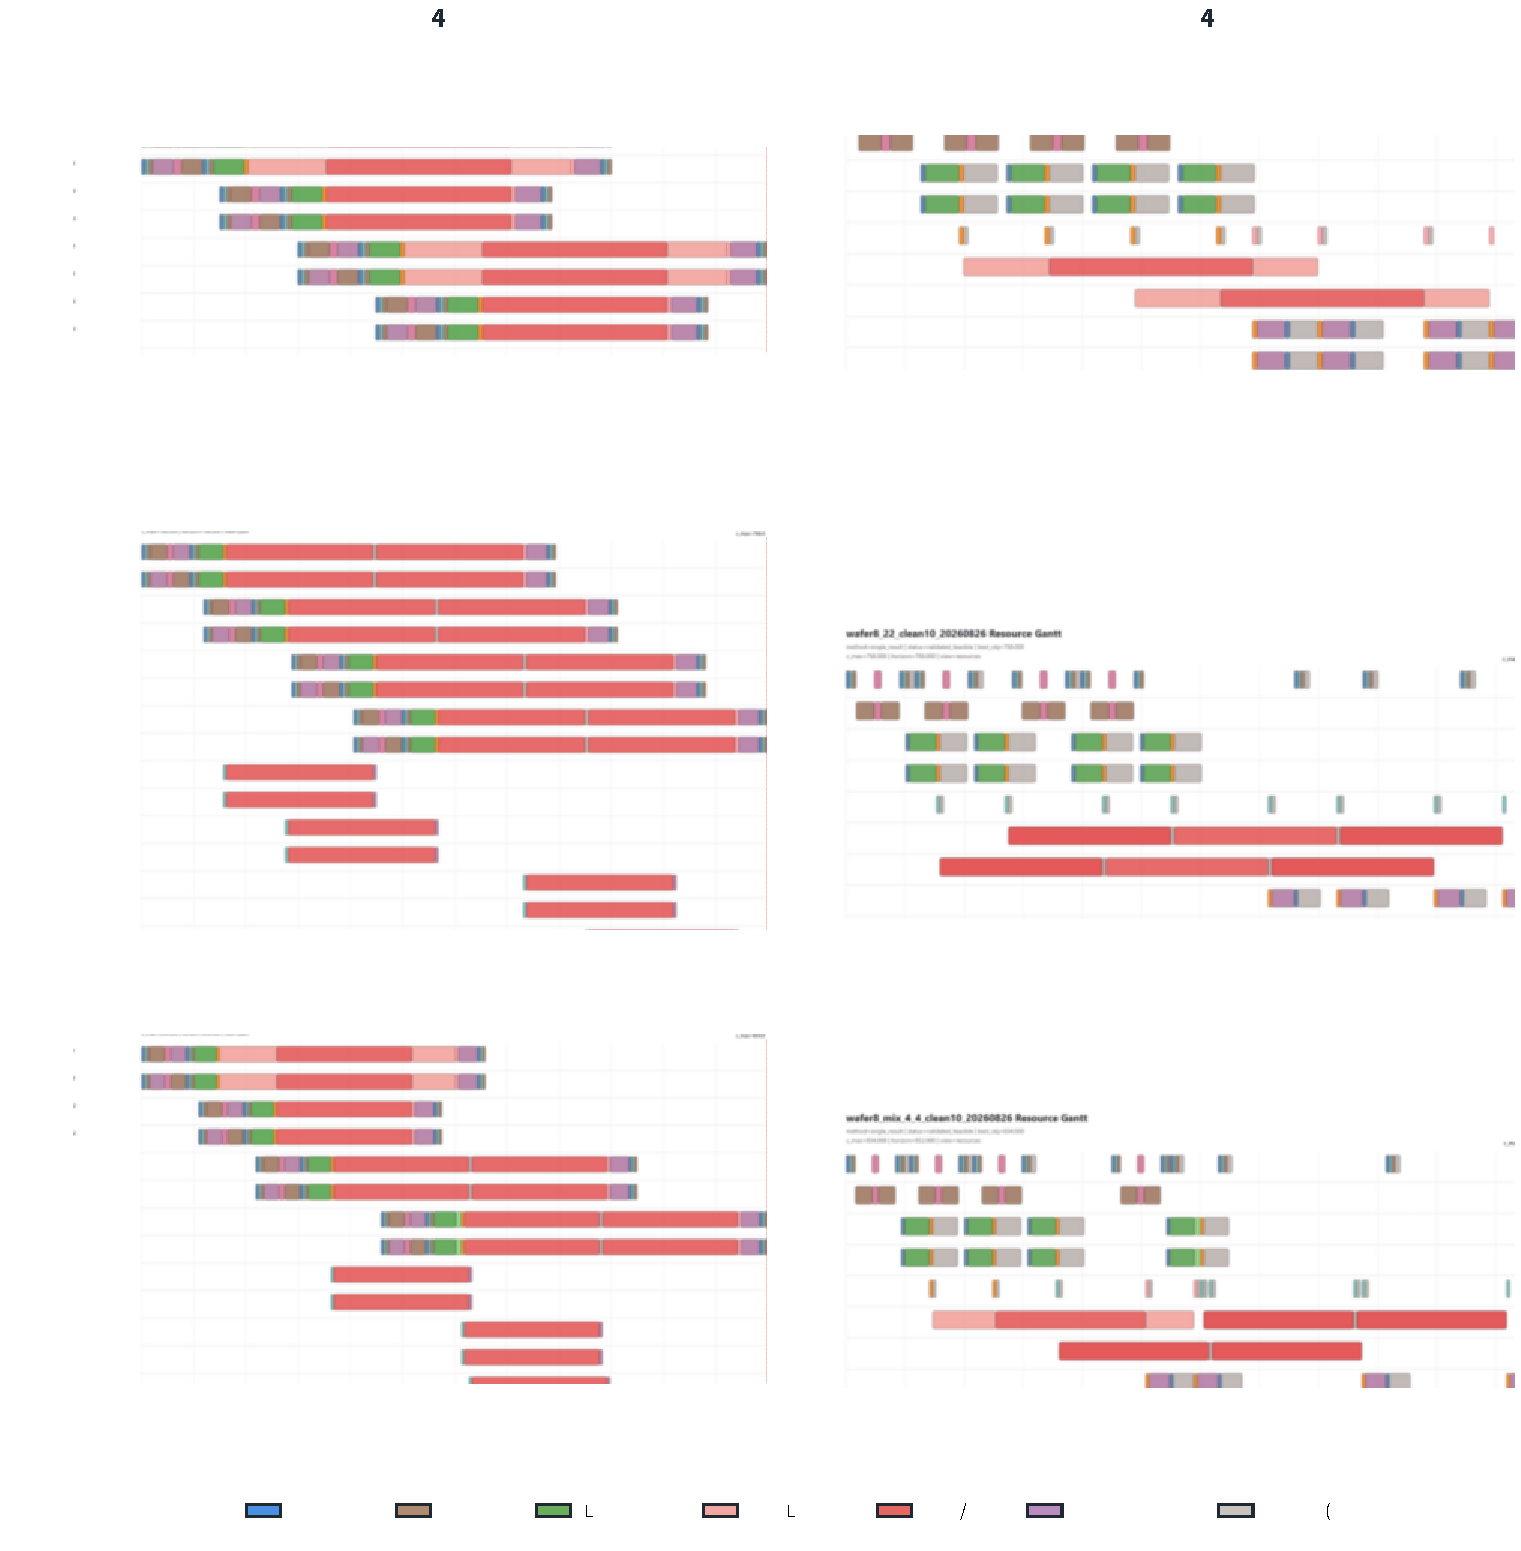
\includegraphics[width=\textwidth]{fig07_mode_gantt8}
\caption{8片实例的最优排程甘特图。三行分别对应纯$4\times1$、纯$2\times2$和4:4混跑，左、右列分别给出晶圆视角与资源视角。横轴为时间（s）；颜色依次表示搬运、AL对准、装载锁操作、腔室装卸片、腔室加工、回片/下游处理以及等待/占位。三种模式的$C_{\max}$分别为610、768和834~s，对应等效吞吐率为47.21、37.50和34.53片/h。}
\label{fig:gantt8-zh}
\end{figure*}

\begin{figure*}[!htbp]
\centering
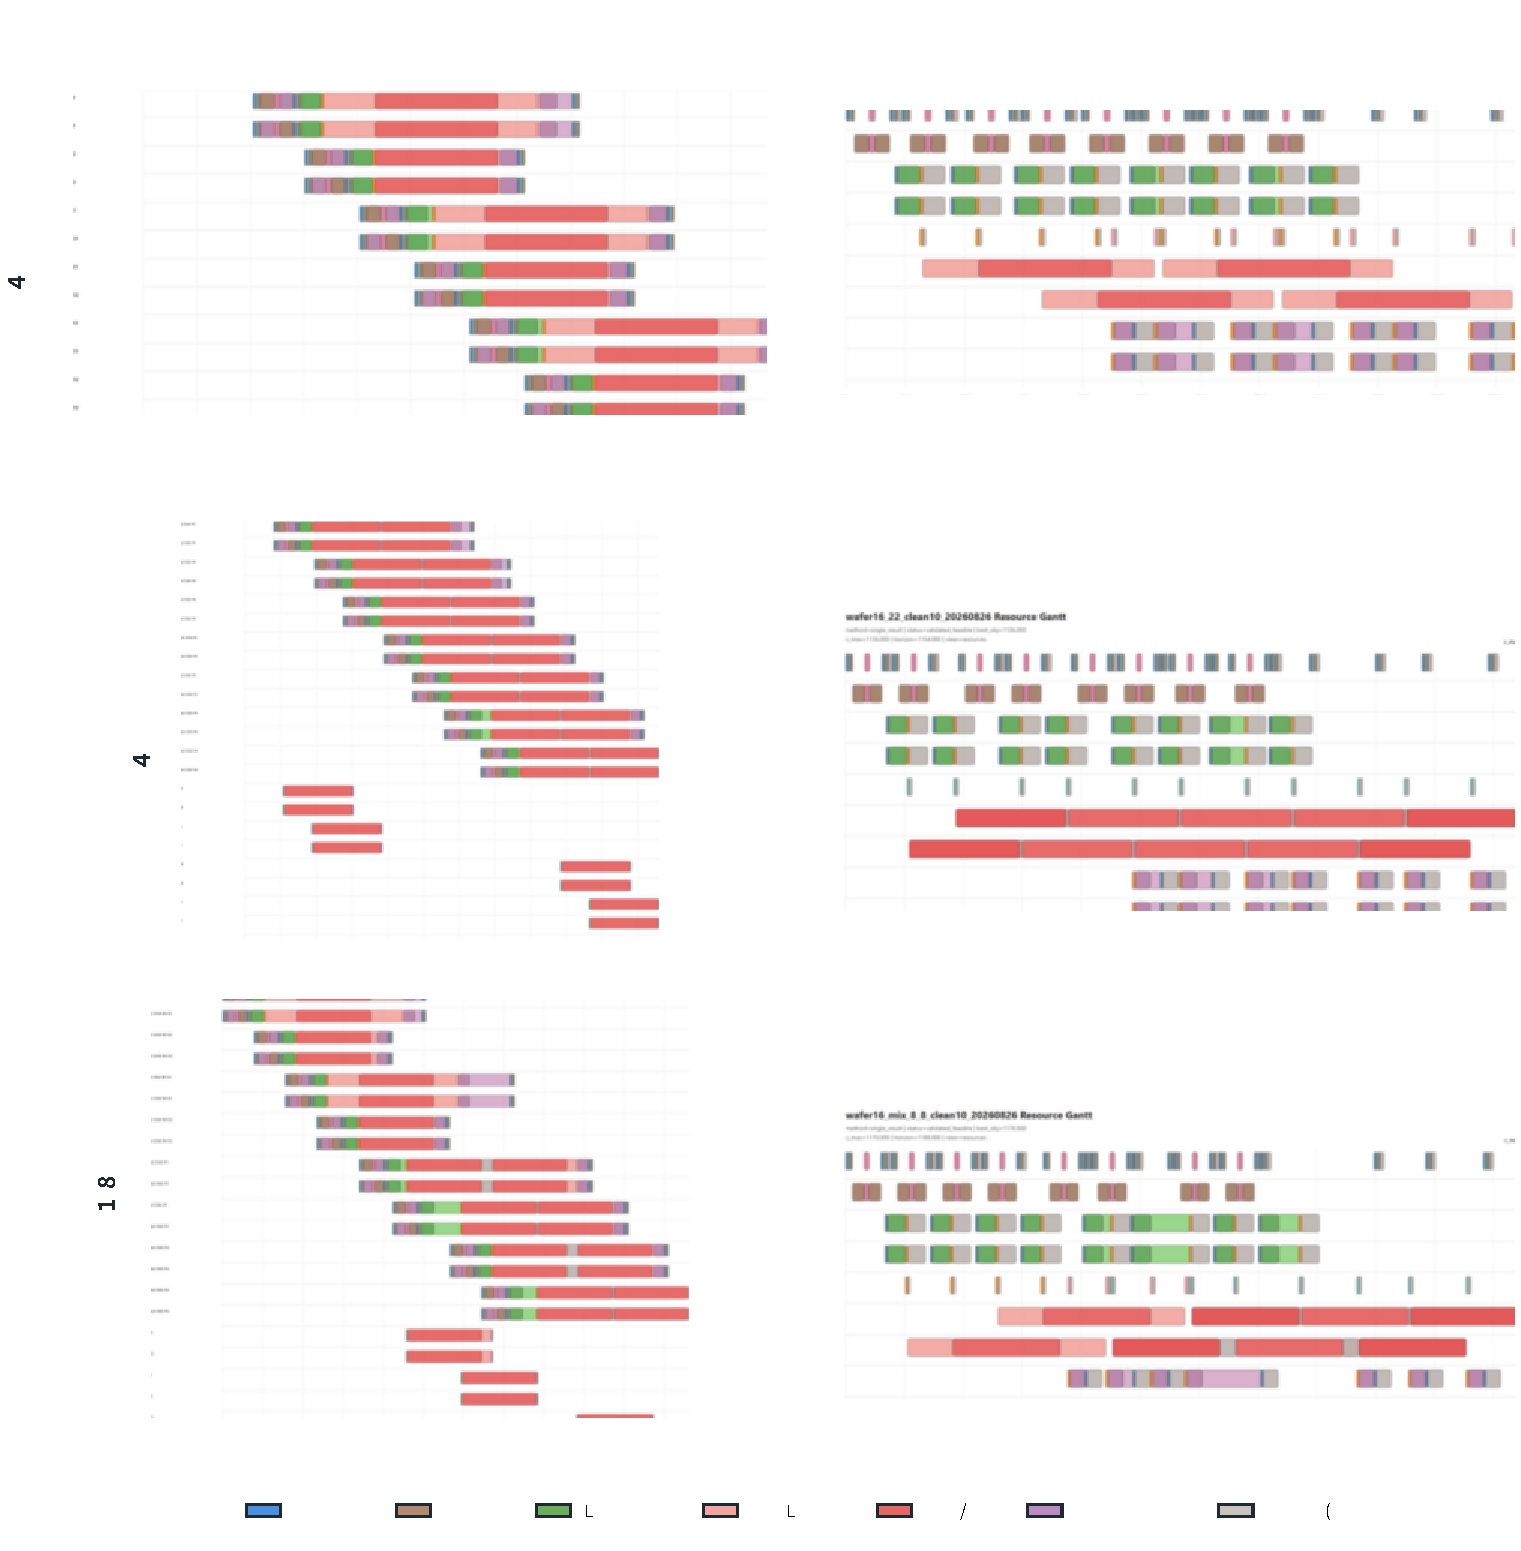
\includegraphics[width=\textwidth]{fig08_mode_gantt16}
\caption{16片实例的最优排程甘特图。三行分别对应纯$4\times1$、纯$2\times2$和8:8混跑，左、右列分别给出晶圆视角与资源视角。横轴为时间（s）；颜色含义与图~\ref{fig:gantt8-zh}一致。三种模式的$C_{\max}$分别为944、1136和1170~s，对应等效吞吐率为61.02、50.70和49.23片/h。}
\label{fig:gantt16-zh}
\end{figure*}

等待时间约束会进一步影响制造系统的产出和控制表现\citep{lee2018waiting}。同为600~s总预算时，完整两阶段工作流采用540~s主求解加至多60~s精修，单阶段对照将600~s全部用于主求解。图~\ref{fig:workflow-zh-new}显示，两阶段工作流的路线总等待、最大等待、节拍变异系数和节拍偏差分别降低51.91\%、68.89\%、39.70\%和94.05\%，四项实例级配对差异经Holm校正后均显著，表明两阶段工作流能够在相同总预算下明显改善排程等待与节拍质量。

二次目标对照与完整线性精修均使用540+至多60~s。线性精修的节拍偏差为22.04，较二次目标的60.18降低63.38\%，该配对差异经Holm校正后显著（$p=0.0377$）；路线总等待、最大等待和节拍变异系数整体接近。结果表明，线性精修在相同预算下能够获得更规则的加工节拍。

\begin{figure}[!htbp]
\centering
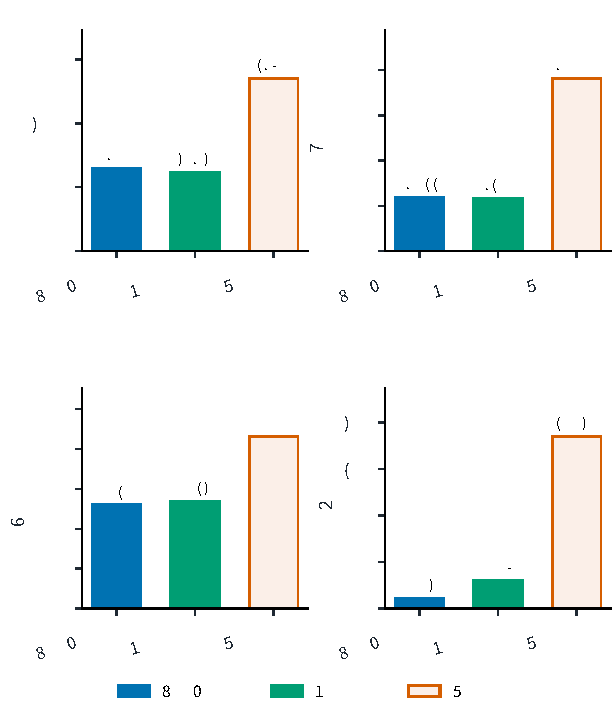
\includegraphics[width=\linewidth]{fig04_workflow_cn}
\caption{相同600~s总预算下的排程运行质量。（a）路线总等待时间；（b）路线最大等待时间；（c）节拍变异系数；（d）节拍偏差。完整两阶段、二次目标对照和单阶段对照分别采用一致的实例集合；纵轴单位依次为s、s、无量纲和s，柱顶为观察均值。}
\label{fig:workflow-zh-new}
\end{figure}

\subsection{SPBS与结构感知割选择}

预计算SPBS的配对实验包含48个实例、每个实例10个配对种子。相对无初始解条件，SPBS将限时内incumbent获得率由51.67\%提高至100\%，增加48.33个百分点（95\%区间$[34.58,62.29]$）；平均PDI由27473.05降至20278.78，降低7194.27或26.19\%（95\%区间$[5145.78,9317.61]$）。两项配对差异经Holm校正后仍显著（$p=2.55\times10^{-5}$和$p=3.46\times10^{-8}$）。结果表明，SPBS能够显著提高限时内完整可行排程的获得率，并改善原始--对偶搜索效率。

\begin{figure}[!htbp]
\centering
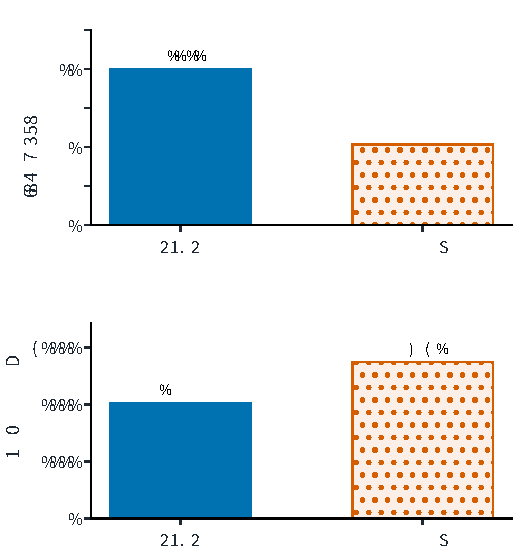
\includegraphics[width=\linewidth]{fig03_spbs_cn}
\caption{SPBS初始解对限时精确搜索的影响。（a）可行incumbent获得率；（b）平均PDI。每个条件包含480次运行；纵轴单位分别为\%和PDI值，柱顶为观察值。}
\label{fig:spbs-zh-new}
\end{figure}

在所有设置共享同一SPBS的2700次标称实验中，比较结构分为三类：纯SCIP作为求解器基线，HEM-13D作为学习型直接基线，\method{}作为完整方法；图中其余条目均为\method{}的组件级消融或单组件变体。消融通过关闭、替换或单独启用自适应评分（adaptive cut scoring，ACS）、束搜索、23维角色感知表示和结构补全等组成部分，检验各模块对有限时间搜索的具体作用及其必要性。所有学习型设置使用相同训练实例、随机种子、候选上限、隐藏维数和求解预算。相对HEM-13D，\method{}的平均PDI由16823.18降至16585.70，降低1.41\%；平均求解时间由219.65~s降至218.32~s，降低0.61\%；平均终止gap由127.24\%降至126.01\%，降低0.97\%；证明最优率由62.4\%提高到63.2\%，增加0.80个百分点。其500次运行全部获得可行解（图~\ref{fig:main-zh-new}）。从HEM的13维表示扩展到23维角色表示带来主要均值改善，随后加入结构补全与束搜索形成完整方法。

\begin{figure}[!htbp]
\centering
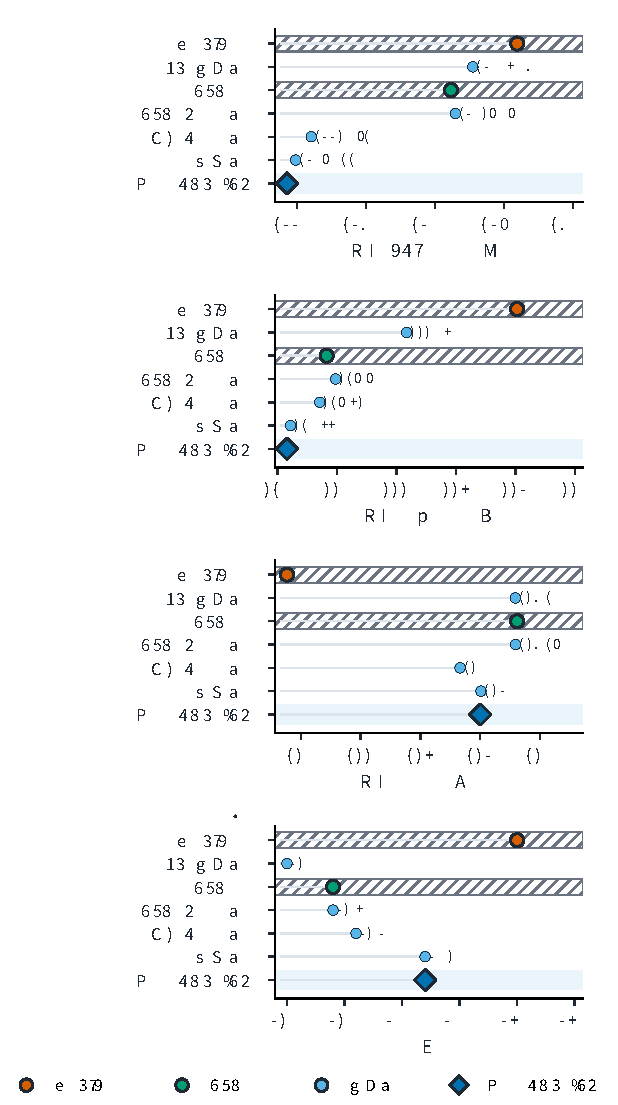
\includegraphics[width=\linewidth]{fig02_nominal_cn}
\caption{共同SPBS条件下的基线与组件消融结果。（a）平均PDI；（b）平均求解时间；（c）平均终止gap；（d）证明最优率。橙色圆、绿色圆、浅蓝色圆和蓝色菱形分别表示纯SCIP基线、HEM-13D基线、组件消融和完整\method{}；横轴单位依次为PDI、s、\%和\%。共2700次运行，点旁标注观察均值。}
\label{fig:main-zh-new}
\end{figure}

以HEM为学习型直接基线，\method{}在PDI、求解时间、终止gap和证明最优率四项指标上均取得改善，并在“两个基线+完整方法+组件消融”的统一实验中取得最低平均PDI和平均求解时间。消融结果表明，23维角色感知表示带来主要均值改善，进一步叠加策略锚定补全与束搜索解码后形成完整方法，并取得最优整体表现。

\subsection{规模、混流构成与求解难度}

析因设计包含$4\times5\times3=60$个晶圆数--配方构成--加工尺度单元，每个单元使用5个求解器种子，共300次运行。图~\ref{fig:doe-zh-new}显示明显的规模转折：8片和16片的75次运行均证明最优，平均PDI分别为28.13和1876.54，平均求解时间为0.34和33.86~s；24片和32片的证明最优率降至36\%和20\%，平均PDI升至31155.94和32959.89，平均求解时间升至408.55和433.20~s。

预设PDI析因模型的$R^2=0.998$。在$1{:}1$混跑条件下，24片和32片的附加交互系数分别为37729.48和40788.63，而加工尺度主效应及其预设交互项的95\%区间均包含0。因此，在所测0.9--1.1加工尺度范围内，求解难度主要由批次规模与混流构成的交互驱动，加工尺度的影响相对较小。

\begin{figure}[!htbp]
\centering
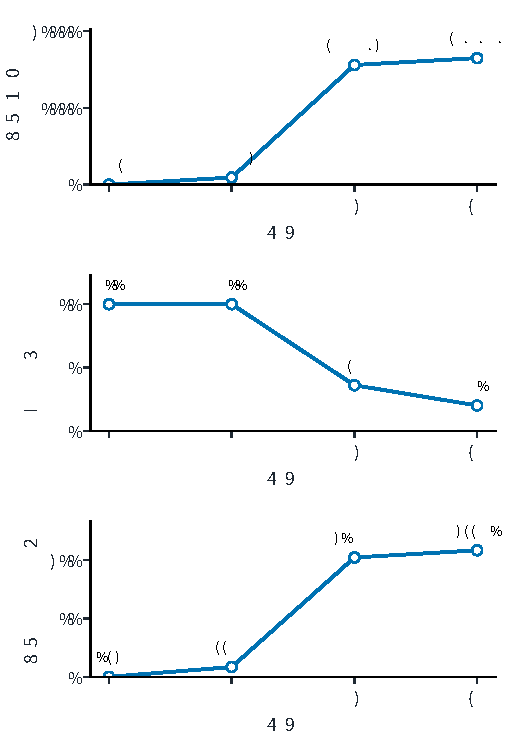
\includegraphics[width=\linewidth]{fig05_doe_cn}
\caption{批次规模对求解性能的影响。（a）平均PDI；（b）证明最优率；（c）平均求解时间。横轴为晶圆数（片），纵轴单位依次为PDI、\%和s；每个规模包含75次运行，共300次运行。}
\label{fig:doe-zh-new}
\end{figure}

\subsection{参数扰动下的可运行性}

既有研究表明，清洗动作及其触发条件会改变CT的机器人动作序列、周期时间和晶圆延迟\citep{yu2020delay,li2022conditioncleaning}。据此，单因素敏感性实验覆盖搬运、加工、清洗间隔和真空区辅助晶圆库存的8个预设场景，共80次运行。全部运行均获得并验解可行排程，其中20次证明最优；场景平均PDI位于28899.41--42478.32之间。较长清洗间隔对应最低平均PDI，较慢搬运对应最高平均PDI，表明清洗频率和共享机械手搬运节拍会明显改变搜索难度；同时，框架在全部预设扰动场景下均稳定获得可行排程。

\subsection{分布偏移下的可行排程交付}

分布偏移测试把批次扩大到40--64片并改变混流组成，9个制造场景共形成729次运行。全部729次运行均返回通过SCIP和独立后处理检查的incumbent，说明所构建的SPBS--MILP--SCIP求解链路在更大规模和分布偏移条件下仍能稳定交付可验证排程。

\begin{figure}[!htbp]
\centering
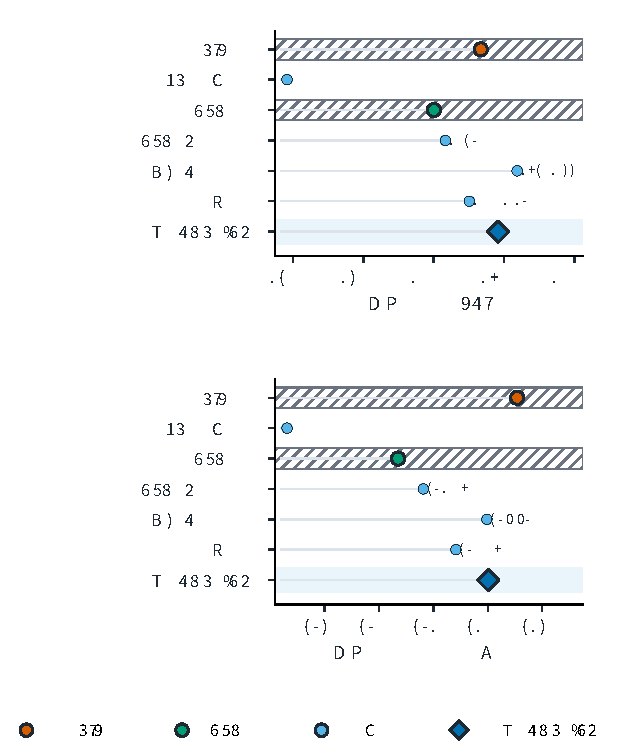
\includegraphics[width=\linewidth]{fig06_ood_cn}
\caption{40--64片分布外测试结果。（a）实例优先平均PDI；（b）平均终止gap。橙色圆、绿色圆、浅蓝色圆和蓝色菱形分别表示纯SCIP基线、HEM-13D基线、组件消融和完整\method{}；横轴单位分别为PDI和\%。共729次运行。}
\label{fig:ood-zh-new}
\end{figure}

在分布偏移实验中，“仅自适应评分”变体取得最低观察平均PDI（70915.54）和终止gap（160.78\%）；完整\method{}的相应数值为73919.15和170.02\%，纯SCIP基线为73670.99和171.35\%。结果说明，在40--64片分布偏移条件下，简单评分组件具有较强鲁棒性；同时，共享SPBS--MILP--SCIP链路在全部729次运行中均稳定获得经检查的可行排程。

\subsection{工业解释与综合结论}

综合实验结果可得到三点工业结论：在配方未限定时，纯$4\times1$在8片和16片批次中具有最高吞吐效率；两阶段工作流在相同总预算下能够显著改善等待与节拍质量；SPBS与结构感知割选择分别从原始可行解和限时搜索轨迹两侧提升求解性能。析因、敏感性和分布偏移实验进一步表明，批次规模与混流构成是求解难度的主要驱动因素，所构建框架能够在参数扰动和40--64片大规模实例上持续交付经检查的可行排程。

\FloatBarrier

\section{结论}

本文面向双源旋转腔半导体组合设备，建立了统一描述$4\times1$并行加工、$2\times2$链式加工、可复用辅助晶圆、清洗和共享搬运的有限时域两阶段MILP，并进一步提出SPBS初始解和结构感知层次割选择方法\method{}。模型以含两个晶圆的PW对为物理搬运与腔室占位单元，统一表示P+P产品PW对、D+D辅助PW对和P+D混合PW对，并明确表达$4\times1$满片批次同步加工一次及$2\times2$中每片产品晶圆在相邻周期加工两次。精确工艺模式比较表明，纯$4\times1$在8片和16片批次中均取得最短最大完工时间和最高等效吞吐率。相同600~s总预算下，两阶段工作流使路线总等待、最大等待、节拍变异系数和节拍偏差分别降低51.91\%、68.89\%、39.70\%和94.05\%。SPBS将限时可行解率由51.67\%提高到100\%，并使平均PDI降低26.19\%；在共同SPBS的基线与消融实验中，以纯SCIP和HEM-13D作为两类基线，组件消融用于验证本方法各组成部分的作用与必要性；相对HEM-13D，\method{}的PDI、求解时间和终止gap分别降低1.41\%、0.61\%和0.97\%，证明最优率提高0.80个百分点。析因实验显示，批次规模与混流构成的交互是求解难度的主要驱动因素；在40--64片分布偏移测试中，729次运行均获得经检查的可行排程。

上述结果表明，将设备结构同时嵌入MILP建模、两阶段运行质量优化、原始初始解构造和割选择，可以兼顾制造排程质量与有限时间精确搜索效率。后续工作将进一步研究随机到达、设备扰动和在线重调度，并评估SPBS构造、滚动优化与产线级部署的整体收益。

\section*{CRediT作者贡献声明}
魏林聪负责概念设计、方法设计、软件实现、验证、形式分析、研究实施、数据管理、可视化、初稿撰写以及审阅与编辑；邵立珍负责概念设计、方法设计、形式分析、验证、审阅与编辑以及项目管理；王蔚负责形式分析、研究实施、审阅与编辑以及监督指导。全体作者审阅并批准最终稿。

\section*{利益冲突声明}
作者声明不存在可能影响本文工作的已知财务利益或个人关系。

\section*{数据与代码可用性}
支撑本文结果的数据、数学实例、训练模型和源代码可向通信作者合理申请。正式发表版
将给出永久公共归档地址。

\section*{稿件准备过程中生成式AI和AI辅助技术的声明}
在本稿准备过程中，作者使用OpenAI ChatGPT和Codex改进语言和可读性、检查LaTeX一致性并辅助软件调试。使用上述工具后，作者按需要审阅和编辑相关内容，并对出版物的全部内容承担责任。

\footnotesize
\setlength{\bibsep}{0pt}
\begin{thebibliography}{32}
\expandafter\ifx\csname natexlab\endcsname\relax\def\natexlab#1{#1}\fi
\providecommand{\url}[1]{\texttt{#1}}
\providecommand{\href}[2]{#2}
\providecommand{\path}[1]{#1}
\providecommand{\DOIprefix}{doi:}
\providecommand{\ArXivprefix}{arXiv:}
\providecommand{\URLprefix}{URL: }
\providecommand{\Pubmedprefix}{pmid:}
\providecommand{\doi}[1]{\href{http://dx.doi.org/#1}{\path{#1}}}
\providecommand{\Pubmed}[1]{\href{pmid:#1}{\path{#1}}}
\providecommand{\bibinfo}[2]{#2}
\ifx\xfnm\relax \def\xfnm[#1]{\unskip,\space#1}\fi
%Type = Article
\bibitem[{Pan et~al.(2018)Pan, Zhou, Qiao and Wu}]{pan2018survey}
\bibinfo{author}{Pan, C.R.}, \bibinfo{author}{Zhou, M.C.},
  \bibinfo{author}{Qiao, Y.}, \bibinfo{author}{Wu, N.Q.},
  \bibinfo{year}{2018}.
\newblock \bibinfo{title}{Scheduling cluster tools in semiconductor manufacturing:
  Recent advances and challenges}.
\newblock \bibinfo{journal}{IEEE Transactions on Automation Science and Engineering}
  \bibinfo{volume}{15}, \bibinfo{number}{2}, \bibinfo{pages}{586--601}.
\newblock \DOIprefix\doi{10.1109/TASE.2016.2642997}.
%Type = Article
\bibitem[{Gu et~al.(2024)Gu, Wu, Qiao, Zhang and Li}]{gu2024applied}
\bibinfo{author}{Gu, L.}, \bibinfo{author}{Wu, N.},
  \bibinfo{author}{Qiao, Y.}, \bibinfo{author}{Zhang, S.},
  \bibinfo{author}{Li, T.}, \bibinfo{year}{2024}.
\newblock \bibinfo{title}{Scheduling cluster tools with multi-space process
  modules and a multi-finger-arm robot in wafer fabrication subject to wafer
  residency time constraints}.
\newblock \bibinfo{journal}{Applied Sciences} \bibinfo{volume}{14},
  \bibinfo{pages}{9490}.
\newblock \DOIprefix\doi{10.3390/app14209490}.
%Type = Article
\bibitem[{Perkinson et~al.(1994)Perkinson, McLarty, Gyurcsik and
  Cavin}]{perkinson1994throughput}
\bibinfo{author}{Perkinson, T.L.}, \bibinfo{author}{McLarty, P.K.},
  \bibinfo{author}{Gyurcsik, R.S.}, \bibinfo{author}{Cavin, R.K.},
  \bibinfo{year}{1994}.
\newblock \bibinfo{title}{Single-wafer cluster tool performance: An analysis
  of throughput}.
\newblock \bibinfo{journal}{IEEE Transactions on Semiconductor Manufacturing}
  \bibinfo{volume}{7}, \bibinfo{pages}{369--373}.
\newblock \DOIprefix\doi{10.1109/66.311340}.
%Type = Article
\bibitem[{Rostami and Hamidzadeh(2002)}]{rostami2002optimal}
\bibinfo{author}{Rostami, S.}, \bibinfo{author}{Hamidzadeh, B.},
  \bibinfo{year}{2002}.
\newblock \bibinfo{title}{Optimal scheduling techniques for cluster tools
  with process-module and transport-module residency constraints}.
\newblock \bibinfo{journal}{IEEE Transactions on Semiconductor Manufacturing}
  \bibinfo{volume}{15}, \bibinfo{pages}{341--349}.
\newblock \DOIprefix\doi{10.1109/TSM.2002.801379}.
%Type = Article
\bibitem[{Wu and Zhou(2010)}]{wu2010closedform}
\bibinfo{author}{Wu, N.Q.}, \bibinfo{author}{Zhou, M.C.},
  \bibinfo{year}{2010}.
\newblock \bibinfo{title}{A closed-form solution for schedulability and
  optimal scheduling of dual-arm cluster tools with wafer residency time
  constraint based on steady schedule analysis}.
\newblock \bibinfo{journal}{IEEE Transactions on Automation Science and
  Engineering} \bibinfo{volume}{7}, \bibinfo{pages}{303--315}.
\newblock \DOIprefix\doi{10.1109/TASE.2008.2008633}.
%Type = Article
\bibitem[{Qiao et~al.(2012)Qiao, Wu and Zhou}]{qiao2012sojourn}
\bibinfo{author}{Qiao, Y.}, \bibinfo{author}{Wu, N.Q.},
  \bibinfo{author}{Zhou, M.C.}, \bibinfo{year}{2012}.
\newblock \bibinfo{title}{Petri net modeling and wafer sojourn time analysis
  of single-arm cluster tools with residency time constraints and activity
  time variation}.
\newblock \bibinfo{journal}{IEEE Transactions on Semiconductor Manufacturing}
  \bibinfo{volume}{25}, \bibinfo{pages}{432--446}.
\newblock \DOIprefix\doi{10.1109/TSM.2012.2199338}.
%Type = Article
\bibitem[{Qiao et~al.(2014)Qiao, Wu and Zhou}]{qiao2014revisiting}
\bibinfo{author}{Qiao, Y.}, \bibinfo{author}{Wu, N.},
  \bibinfo{author}{Zhou, M.C.}, \bibinfo{year}{2014}.
\newblock \bibinfo{title}{Scheduling of dual-arm cluster tools with wafer
  revisiting and residency time constraints}.
\newblock \bibinfo{journal}{IEEE Transactions on Industrial Informatics}
  \bibinfo{volume}{10}, \bibinfo{pages}{286--300}.
\newblock \DOIprefix\doi{10.1109/TII.2013.2272702}.
%Type = Article
\bibitem[{Wang et~al.(2020)Wang, Hu, Pan, Zhou and Li}]{wang2020multiple}
\bibinfo{author}{Wang, J.}, \bibinfo{author}{Hu, H.},
  \bibinfo{author}{Pan, C.}, \bibinfo{author}{Zhou, Y.},
  \bibinfo{author}{Li, L.}, \bibinfo{year}{2020}.
\newblock \bibinfo{title}{Scheduling dual-arm cluster tools with multiple
  wafer types and residency time constraints}.
\newblock \bibinfo{journal}{IEEE/CAA Journal of Automatica Sinica}
  \bibinfo{volume}{7}, \bibinfo{pages}{776--789}.
\newblock \DOIprefix\doi{10.1109/JAS.2020.1003150}.
%Type = Article
\bibitem[{Wang et~al.(2025)Wang, Liu, Zhou and
  Abusorrah}]{wang2025virtualcell}
\bibinfo{author}{Wang, J.}, \bibinfo{author}{Liu, C.},
  \bibinfo{author}{Zhou, M.C.}, \bibinfo{author}{Abusorrah, A.},
  \bibinfo{year}{2025}.
\newblock \bibinfo{title}{Virtual cell-based scheduling approach to
  single-robotic-arm cluster tools subject to wafer residency time
  constraints}.
\newblock \bibinfo{journal}{IEEE Transactions on Automation Science and
  Engineering} \bibinfo{volume}{22}, \bibinfo{pages}{240--251}.
\newblock \DOIprefix\doi{10.1109/TASE.2024.3349380}.
%Type = Article
\bibitem[{Lee et~al.(2018)Lee, Zhao, Li and Papadopoulos}]{lee2018waiting}
\bibinfo{author}{Lee, J.H.}, \bibinfo{author}{Zhao, C.},
  \bibinfo{author}{Li, J.}, \bibinfo{author}{Papadopoulos, C.T.},
  \bibinfo{year}{2018}.
\newblock \bibinfo{title}{Analysis, design, and control of {Bernoulli}
  production lines with waiting time constraints}.
\newblock \bibinfo{journal}{Journal of Manufacturing Systems}
  \bibinfo{volume}{46}, \bibinfo{pages}{208--220}.
\newblock \DOIprefix\doi{10.1016/j.jmsy.2018.01.001}.
%Type = Article
\bibitem[{Zhu et~al.(2025)Zhu, Yuan, Wang and Hou}]{zhu2025failuredeadlock}
\bibinfo{author}{Zhu, Q.}, \bibinfo{author}{Yuan, J.},
  \bibinfo{author}{Wang, G.}, \bibinfo{author}{Hou, Y.}, \bibinfo{year}{2025}.
\newblock \bibinfo{title}{Scheduling a single-arm two-cluster tool with a
  process module failure subject to wafer residency time constraints}.
\newblock \bibinfo{journal}{IEEE Transactions on Automation Science and
  Engineering} \bibinfo{volume}{22}, \bibinfo{pages}{667--679}.
\newblock \DOIprefix\doi{10.1109/TASE.2023.3275703}.
%Type = Article
\bibitem[{Kim and Kim(2025)}]{kim2025noncyclicdeadlock}
\bibinfo{author}{Kim, D.}, \bibinfo{author}{Kim, H.J.}, \bibinfo{year}{2025}.
\newblock \bibinfo{title}{Noncyclic scheduling of cluster tools using deep
  reinforcement learning}.
\newblock \bibinfo{journal}{IEEE Transactions on Automation Science and
  Engineering} \bibinfo{volume}{22}, \bibinfo{pages}{24009--24023}.
\newblock \DOIprefix\doi{10.1109/TASE.2025.3632534}.
%Type = Article
\bibitem[{Kim et~al.(2013)Kim, Kim, Lee and Lee}]{kim2013cleaning}
\bibinfo{author}{Kim, H.}, \bibinfo{author}{Kim, H.J.},
  \bibinfo{author}{Lee, J.H.}, \bibinfo{author}{Lee, T.E.},
  \bibinfo{year}{2013}.
\newblock \bibinfo{title}{Scheduling dual-armed cluster tools with cleaning
  processes}.
\newblock \bibinfo{journal}{International Journal of Production Research}
  \bibinfo{volume}{51}, \bibinfo{pages}{3671--3687}.
\newblock \DOIprefix\doi{10.1080/00207543.2012.758392}.
%Type = Article
\bibitem[{Yu and Lee(2020)}]{yu2020delay}
\bibinfo{author}{Yu, T.S.}, \bibinfo{author}{Lee, T.E.},
  \bibinfo{year}{2020}.
\newblock \bibinfo{title}{Wafer delay analysis and control of dual-armed
  cluster tools with chamber cleaning operations}.
\newblock \bibinfo{journal}{International Journal of Production Research}
  \bibinfo{volume}{58}, \bibinfo{pages}{434--447}.
\newblock \DOIprefix\doi{10.1080/00207543.2019.1593547}.
%Type = Article
\bibitem[{Qiao et~al.(2022)Qiao, Lu, Li, Zhang, Wu and Liu}]{qiao2022binary}
\bibinfo{author}{Qiao, Y.}, \bibinfo{author}{Lu, Y.}, \bibinfo{author}{Li, J.},
  \bibinfo{author}{Zhang, S.}, \bibinfo{author}{Wu, N.}, \bibinfo{author}{Liu,
  B.}, \bibinfo{year}{2022}.
\newblock \bibinfo{title}{An efficient binary integer programming model for
  residency time-constrained cluster tools with chamber cleaning requirements}.
\newblock \bibinfo{journal}{IEEE Transactions on Automation Science and
  Engineering} \bibinfo{volume}{19}, \bibinfo{pages}{1757--1771}.
\newblock \DOIprefix\doi{10.1109/TASE.2021.3122576}.
%Type = Article
\bibitem[{Li et~al.(2022)Li, Yang and Zhen}]{li2022conditioncleaning}
\bibinfo{author}{Li, C.}, \bibinfo{author}{Yang, F.}, \bibinfo{author}{Zhen,
  L.}, \bibinfo{year}{2022}.
\newblock \bibinfo{title}{Efficient scheduling approaches to time-constrained
  single-armed cluster tools with condition-based chamber cleaning operations}.
\newblock \bibinfo{journal}{International Journal of Production Research}
  \bibinfo{volume}{60}, \bibinfo{pages}{3555--3568}.
\newblock \DOIprefix\doi{10.1080/00207543.2021.1926568}.
%Type = Inproceedings
\bibitem[{Gu et~al.(2024)Gu, Wu, Qiao and Zhang}]{gu2024multifinger}
\bibinfo{author}{Gu, L.}, \bibinfo{author}{Wu, N.}, \bibinfo{author}{Qiao, Y.},
  \bibinfo{author}{Zhang, S.}, \bibinfo{year}{2024}.
\newblock \bibinfo{title}{Scheduling of {Multi-finger-robotic Cluster Tools}
  with {Multi-space Process Modules}}, in: \bibinfo{booktitle}{2024
  International Conference on Networking, Sensing and Control ({ICNSC})},
  \bibinfo{publisher}{IEEE}.
\newblock \DOIprefix\doi{10.1109/ICNSC62968.2024.10760109}.
%Type = Article
\bibitem[{Yang et~al.(2025)Yang, Li, Zhen, Zhang and Wu}]{yang2025miptwowafers}
\bibinfo{author}{Yang, F.}, \bibinfo{author}{Li, C.}, \bibinfo{author}{Zhen,
  L.}, \bibinfo{author}{Zhang, C.}, \bibinfo{author}{Wu, N.},
  \bibinfo{year}{2025}.
\newblock \bibinfo{title}{Scheduling residency time-constrained single-armed
  cluster tools with two-wafer types via mixed integer programming model}.
\newblock \bibinfo{journal}{Expert Systems with Applications}
  \bibinfo{volume}{288}, \bibinfo{pages}{128209}.
\newblock \DOIprefix\doi{10.1016/j.eswa.2025.128209}.
%Type = Article
\bibitem[{Kim and Lee(2025)}]{kim2025adaptivecluster}
\bibinfo{author}{Kim, H.J.}, \bibinfo{author}{Lee, J.H.}, \bibinfo{year}{2025}.
\newblock \bibinfo{title}{Scheduling cluster tools for concurrent processing:
  Deep reinforcement learning with adaptive search}.
\newblock \bibinfo{journal}{IEEE Transactions on Automation Science and
  Engineering} \bibinfo{volume}{22}, \bibinfo{pages}{3783--3796}.
\newblock \DOIprefix\doi{10.1109/TASE.2024.3399818}.
%Type = Article
\bibitem[{Hong et~al.(2026)Hong, Hsu and Chen}]{hong2026ddpgct}
\bibinfo{author}{Hong, T.Y.}, \bibinfo{author}{Hsu, C.Y.},
  \bibinfo{author}{Chen, C.L.}, \bibinfo{year}{2026}.
\newblock \bibinfo{title}{Simulation-based deep reinforcement learning for
  process time optimization in semiconductor cluster tool and an empirical
  study}.
\newblock \bibinfo{journal}{Computers \& Industrial Engineering}
  \bibinfo{volume}{211}, \bibinfo{pages}{111698}.
\newblock \DOIprefix\doi{10.1016/j.cie.2025.111698}.
%Type = Inproceedings
\bibitem[{Tang et~al.(2020)Tang, Agrawal and Faenza}]{tang2020cut}
\bibinfo{author}{Tang, Y.}, \bibinfo{author}{Agrawal, S.},
  \bibinfo{author}{Faenza, Y.}, \bibinfo{year}{2020}.
\newblock \bibinfo{title}{Reinforcement learning for integer programming:
  Learning to cut}, in: \bibinfo{booktitle}{Proceedings of the 37th
  International Conference on Machine Learning}, \bibinfo{publisher}{PMLR}. pp.
  \bibinfo{pages}{9367--9376}.
\newblock \URLprefix \url{https://proceedings.mlr.press/v119/tang20a.html}.
%Type = Article
\bibitem[{Huang et~al.(2022)Huang, Wang, Liu, Zhen, Zhang, Yuan, Hao, Yu and
  Wang}]{huang2022cutranking}
\bibinfo{author}{Huang, Z.}, \bibinfo{author}{Wang, K.}, \bibinfo{author}{Liu,
  F.}, \bibinfo{author}{Zhen, H.L.}, \bibinfo{author}{Zhang, W.},
  \bibinfo{author}{Yuan, M.}, \bibinfo{author}{Hao, J.}, \bibinfo{author}{Yu,
  Y.}, \bibinfo{author}{Wang, J.}, \bibinfo{year}{2022}.
\newblock \bibinfo{title}{Learning to select cuts for efficient mixed-integer
  programming}.
\newblock \bibinfo{journal}{Pattern Recognition} \bibinfo{volume}{123},
  \bibinfo{pages}{108353}.
\newblock \DOIprefix\doi{10.1016/j.patcog.2021.108353}.
%Type = Inproceedings
\bibitem[{Paulus et~al.(2022)Paulus, Zarpellon, Krause, Charlin and
  Maddison}]{paulus2022looking}
\bibinfo{author}{Paulus, M.B.}, \bibinfo{author}{Zarpellon, G.},
  \bibinfo{author}{Krause, A.}, \bibinfo{author}{Charlin, L.},
  \bibinfo{author}{Maddison, C.}, \bibinfo{year}{2022}.
\newblock \bibinfo{title}{Learning to cut by looking ahead: Cutting plane
  selection via imitation learning}, in: \bibinfo{booktitle}{Proceedings of the
  39th International Conference on Machine Learning},
  \bibinfo{publisher}{PMLR}. pp. \bibinfo{pages}{17584--17600}.
\newblock \URLprefix \url{https://proceedings.mlr.press/v162/paulus22a.html}.
%Type = Inproceedings
\bibitem[{Wang et~al.(2023b)Wang, Li, Wang, Kuang, Yuan, Zeng, Zhang and
  Wu}]{wang2023hem}
\bibinfo{author}{Wang, Z.}, \bibinfo{author}{Li, X.}, \bibinfo{author}{Wang,
  J.}, \bibinfo{author}{Kuang, Y.}, \bibinfo{author}{Yuan, M.},
  \bibinfo{author}{Zeng, J.}, \bibinfo{author}{Zhang, Y.}, \bibinfo{author}{Wu,
  F.}, \bibinfo{year}{2023}b.
\newblock \bibinfo{title}{Learning cut selection for mixed-integer linear
  programming via hierarchical sequence model}, in:
  \bibinfo{booktitle}{Proceedings of the Eleventh International Conference on
  Learning Representations}.
\newblock \URLprefix \url{https://openreview.net/forum?id=Zob4P9bRNcK}.
%Type = Article
\bibitem[{Achterberg(2009)}]{achterberg2009scip}
\bibinfo{author}{Achterberg, T.}, \bibinfo{year}{2009}.
\newblock \bibinfo{title}{{SCIP}: Solving constraint integer programs}.
\newblock \bibinfo{journal}{Mathematical Programming Computation}
  \bibinfo{volume}{1}, \bibinfo{pages}{1--41}.
\newblock \DOIprefix\doi{10.1007/s12532-008-0001-1}.
%Type = Article
\bibitem[{Bestuzheva et~al.(2023)Bestuzheva, Besan{\c{c}}on, Chen, Chmiela,
  Donkiewicz, van Doornmalen, Eifler, Gaul, Gamrath, Gleixner, Gottwald,
  Graczyk, Halbig, Hoen, Hojny, van~der Hulst, Koch, L{\"u}bbecke, Maher,
  Matter, M{\"u}hmer, M{\"u}ller, Pfetsch, Schl{\"o}sser, Serrano, Shinano,
  Sofranac, Turner, Vigerske, Wegscheider, Wellner, Weninger and
  Witzig}]{bestuzheva2023scip}
\bibinfo{author}{Bestuzheva, K.}, \bibinfo{author}{Besan{\c{c}}on, M.},
  \bibinfo{author}{Chen, W.K.}, \bibinfo{author}{Chmiela, A.},
  \bibinfo{author}{Donkiewicz, T.}, \bibinfo{author}{van Doornmalen, J.},
  \bibinfo{author}{Eifler, L.}, \bibinfo{author}{Gaul, O.},
  \bibinfo{author}{Gamrath, G.}, \bibinfo{author}{Gleixner, A.},
  \bibinfo{author}{Gottwald, L.}, \bibinfo{author}{Graczyk, C.},
  \bibinfo{author}{Halbig, K.}, \bibinfo{author}{Hoen, A.},
  \bibinfo{author}{Hojny, C.}, \bibinfo{author}{van~der Hulst, R.},
  \bibinfo{author}{Koch, T.}, \bibinfo{author}{L{\"u}bbecke, M.E.},
  \bibinfo{author}{Maher, S.J.}, \bibinfo{author}{Matter, F.},
  \bibinfo{author}{M{\"u}hmer, E.}, \bibinfo{author}{M{\"u}ller, B.},
  \bibinfo{author}{Pfetsch, M.E.}, \bibinfo{author}{Schl{\"o}sser, F.},
  \bibinfo{author}{Serrano, F.}, \bibinfo{author}{Shinano, Y.},
  \bibinfo{author}{Sofranac, B.}, \bibinfo{author}{Turner, M.},
  \bibinfo{author}{Vigerske, S.}, \bibinfo{author}{Wegscheider, F.},
  \bibinfo{author}{Wellner, P.}, \bibinfo{author}{Weninger, D.},
  \bibinfo{author}{Witzig, J.}, \bibinfo{year}{2023}.
\newblock \bibinfo{title}{Enabling research through the {SCIP} optimization
  suite 8.0}.
\newblock \bibinfo{journal}{ACM Transactions on Mathematical Software}
  \bibinfo{volume}{49}, \bibinfo{pages}{22:1--22:21}.
\newblock \DOIprefix\doi{10.1145/3585516}.
%Type = Inproceedings
\bibitem[{Vinyals et~al.(2015)Vinyals, Fortunato and
  Jaitly}]{vinyals2015pointer}
\bibinfo{author}{Vinyals, O.}, \bibinfo{author}{Fortunato, M.},
  \bibinfo{author}{Jaitly, N.}, \bibinfo{year}{2015}.
\newblock \bibinfo{title}{Pointer networks}, in: \bibinfo{booktitle}{Advances
  in Neural Information Processing Systems}, pp. \bibinfo{pages}{2692--2700}.
%Type = Inproceedings
\bibitem[{Choo et~al.(2022)Choo, Kwon, Kim, Jae, Hottung, Tierney and
  Gwon}]{choo2022beam}
\bibinfo{author}{Choo, J.}, \bibinfo{author}{Kwon, Y.D.}, \bibinfo{author}{Kim,
  J.}, \bibinfo{author}{Jae, J.}, \bibinfo{author}{Hottung, A.},
  \bibinfo{author}{Tierney, K.}, \bibinfo{author}{Gwon, Y.},
  \bibinfo{year}{2022}.
\newblock \bibinfo{title}{Simulation-guided beam search for neural
  combinatorial optimization}, in: \bibinfo{booktitle}{Advances in Neural
  Information Processing Systems}.
\newblock \URLprefix
  \url{https://papers.nips.cc/paper_files/paper/2022/hash/39b9b60f0d149eabd1fff2d7c7d5afc4-Abstract-Conference.html},
  \DOIprefix\doi{10.52202/068431-0637}.
%Type = Article
\bibitem[{Nemhauser et~al.(1978)Nemhauser, Wolsey and
  Fisher}]{nemhauser1978analysis}
\bibinfo{author}{Nemhauser, G.L.}, \bibinfo{author}{Wolsey, L.A.},
  \bibinfo{author}{Fisher, M.L.}, \bibinfo{year}{1978}.
\newblock \bibinfo{title}{An analysis of approximations for maximizing
  submodular set functions---i}.
\newblock \bibinfo{journal}{Mathematical Programming} \bibinfo{volume}{14},
  \bibinfo{pages}{265--294}.
\newblock \DOIprefix\doi{10.1007/BF01588971}.
%Type = Article
\bibitem[{Williams(1992)}]{williams1992reinforce}
\bibinfo{author}{Williams, R.J.}, \bibinfo{year}{1992}.
\newblock \bibinfo{title}{Simple statistical gradient-following algorithms for
  connectionist reinforcement learning}.
\newblock \bibinfo{journal}{Machine Learning} \bibinfo{volume}{8},
  \bibinfo{pages}{229--256}.
\newblock \DOIprefix\doi{10.1007/BF00992696}.
%Type = Inproceedings
\bibitem[{Mnih et~al.(2016)Mnih, Badia, Mirza, Graves, Lillicrap, Harley,
  Silver and Kavukcuoglu}]{mnih2016a3c}
\bibinfo{author}{Mnih, V.}, \bibinfo{author}{Badia, A.P.},
  \bibinfo{author}{Mirza, M.}, \bibinfo{author}{Graves, A.},
  \bibinfo{author}{Lillicrap, T.P.}, \bibinfo{author}{Harley, T.},
  \bibinfo{author}{Silver, D.}, \bibinfo{author}{Kavukcuoglu, K.},
  \bibinfo{year}{2016}.
\newblock \bibinfo{title}{Asynchronous methods for deep reinforcement
  learning}, in: \bibinfo{booktitle}{Proceedings of the 33rd International
  Conference on Machine Learning}, \bibinfo{publisher}{PMLR}. pp.
  \bibinfo{pages}{1928--1937}.
\newblock \URLprefix \url{https://proceedings.mlr.press/v48/mniha16.html}.
%Type = Article
\bibitem[{Gleixner et~al.(2021)Gleixner, Hendel, Gamrath, Achterberg, Bastubbe,
  Berthold, Christophel, Jarck, Koch, Linderoth, Lubbecke, Mittelmann, Ozyurt,
  Ralphs, Salvagnin and Shinano}]{gleixner2021miplib}
\bibinfo{author}{Gleixner, A.}, \bibinfo{author}{Hendel, G.},
  \bibinfo{author}{Gamrath, G.}, \bibinfo{author}{Achterberg, T.},
  \bibinfo{author}{Bastubbe, M.}, \bibinfo{author}{Berthold, T.},
  \bibinfo{author}{Christophel, P.}, \bibinfo{author}{Jarck, K.},
  \bibinfo{author}{Koch, T.}, \bibinfo{author}{Linderoth, J.},
  \bibinfo{author}{Lubbecke, M.E.}, \bibinfo{author}{Mittelmann, H.D.},
  \bibinfo{author}{Ozyurt, D.}, \bibinfo{author}{Ralphs, T.K.},
  \bibinfo{author}{Salvagnin, D.}, \bibinfo{author}{Shinano, Y.},
  \bibinfo{year}{2021}.
\newblock \bibinfo{title}{{MIPLIB} 2017: Data-driven compilation of the 6th
  mixed-integer programming library}.
\newblock \bibinfo{journal}{Mathematical Programming Computation}
  \bibinfo{volume}{13}, \bibinfo{pages}{443--490}.
\newblock \DOIprefix\doi{10.1007/s12532-020-00194-3}.
\end{thebibliography}

\end{document}
